\cotefile{84}
\scanpage{146}
% position: top
\[
T_1\unsure{\Leftarrow|=}\deleted{\unsure{2\varphi}}\unsure{1_1},-b_1
=\deleted{\unsure{T_1}}\begin{pmatrix}2&0\\-b_1&0\end{pmatrix}
\qquad
\unsure{\overline{T}_1|\overline{\tau}_1}
=\begin{pmatrix}0&0\\b_1&2\end{pmatrix}
\]
\deleted{\(\unsure{q_1}\)}
\figure{\begin{tikzpicture}
\node[draw,ellipse,inner sep=4pt] at (0,0) {$b=b_1b_2$};
\end{tikzpicture}}
% position: upper middle
\diagram{\begin{tikzcd}[column sep=large,row sep=large]
(E_1,\deleted{\unsure{q}}\unsure{\xi_1|\beta_1}),(E,\unsure{\xi_2|\beta_2})
\arrow[r] \arrow[d,"\unsure{\mathrm{triv.}}"']
& (E,\unsure{\xi|\beta})\quad\deleted{\text{avec}}\\
\deleted{b_1=E_1}&\deleted{\unsure{E_1}\longrightarrow}\,.
\end{tikzcd}}
\[
\hspace{6em}b_1\qquad b_2
\]
% position: middle left
\diagram{\begin{tikzcd}[column sep=large]
b_1:\ \unsure{M_1}\arrow[r,"\unsure{\tau_1^{\bullet}|\tau'_1}"]&E_1\arrow[r,"\pi_1"]&L_1\\
-b_1:\ M_1\arrow[r,"\unsure{\sigma_1}"]&E_1\arrow[r,"\unsure{\tau_{1\bullet}|\tau_1}"]&L_1
\end{tikzcd}}
% position: middle right
\diagram{$\begin{array}{c|c}
\unsure{\xi'_1|\xi_1}=\unsure{\xi_1|\beta_1}+u_1
&\unsure{\xi'_2|\xi'_1}=\unsure{\xi_2|\beta_2}+u_2\\
b'_1=b_1+\unsure{\chi|\gamma}u_1&b'_2=b_2+\unsure{\chi|\gamma}u_2
\end{array}$}
\[
\unsure{u_i\in\operatorname{Hom}(M_i,L_i)}
\]
% position: lower left
\diagram{$\begin{array}{ll}
\text{\unsure{trivialisations}}&\unsure{\xi}\\
\text{\unsure{quasi-trivialisations}}&\unsure{\beta}
\end{array}$}
\[
\unsure{b_\xi}\qquad
\unsure{\beta_\bullet(\xi)}=b\in\unsure{\operatorname{Hom}}(M_1,L_1)
\]
\[
\unsure{\beta(\varphi)}=-b
\]
% position: lower right
\diagram{\begin{tikzcd}[column sep=huge]
x_1\arrow[r,Rightarrow]&\pi_1(\unsure{\tau'_1}(x_1))\\
x_1\arrow[r,mapsto,dash]&\pi_1(\unsure{\tau_i\cdot u_1}+u_1(x_1))
=\pi_1(\unsure{\tau_i\cdot u_1})
\end{tikzcd}}
% position: foot
\margin{145}

\scanpage{147}
\mspage{475}
% position: upper paragraph
Si quelque chose ici sort du commun, ce n'est pas bien sûr la simple
\mbox{p r é s e n c e} de ce double mécanisme, ni non plus (il me semble) la force de
la composante ``répressive'' à proprement parler, la force donc de la répression
des traits, attitudes, pulsions ``yin''. Il n'y a pas de commune mesure ici avec
ce qui avait lieu chez ma mère, dont la vie (et celle de ses proches) a été dé-\linebreak
vastée par sa haine (restée occulte sa vie durant) de ce qui faisait d'elle une
femme. A aucun moment, je crois, mes façons d'être n'ont été entièrement \unsure{exempte|exemptes}
d'une certaine douceur, voire de tendresse, qui obstinément arrondissaient les
angles du personnage que je m'étais taillé depuis mon enfance, et qui \unsure{m'attiraie|m'attiraient}
souvent sympathie et affection. Le côté exceptionnel se trouverait plutôt dans \unsure{l|la}
\mbox{d é m e s u r e} de mes investissements, dans la démesure de l'énergie que j'in\linebreak
vestis dans mes tâches, sans m'en laisser distraire par un regard à droite ni à
gauche! En dehors du travail proprement dit, mon esprit continuellement est pro-\linebreak
jeté vers l'accomplissement, vers l'aboutissement de telle ou telle étape du tra\linebreak
vail. Cette attitude-là (``Zielgerichtetheit'' en allemand, ``aimdirectedness'' en
anglais) est par excellence une attitude yang, une attitude de \mbox{t e n s i o n},
de \mbox{f e r m e t u r e} à tout ce qui n'apparaît pas directement lié à la tâche

% position: middle paragraph
Cette démesure était de nature à susciter en autrui l'image d'une sorte de
``super-man'' ou ``super-mâle'', admirable certes hélas! (vu les valeurs qui ont
cours), mais suscitant aussitôt (à un niveau qui reste inconscient le plus sou-\linebreak
vent) d'instinctives réactions de défense voire d'antagonisme devant un tel dé-\linebreak
ployement de force, ressenti comme menaçant voire agressif, ou en tous cas dan-\linebreak
gereux \(({}^{108}2)\). Et surtout, cette image irrésistiblement évoque l'image du
``\mbox{s u p e r - p è r e}'', et met en branle aussitôt la multiplicité ambiguë des
réactions d'attraction et de répulsion nouées autour du sempiternel conflit au
père... C'est là \mbox{m a} contribution dans ces relations d' \mbox{a m b i g u i t é},
qui ont été si communes dans ma vie, et auxquelles je me suis retrouvé confronté
tant de fois au cours de Récoltes et Semailles. Cette ambiguïté est renforcée,
non diminuée, par la persistance de traits yin en moi qui alimentent une sympa-\linebreak
thie, que la seule hypertrophie des traits yang en une sorte de gigantesque
``superman'' serait impuissante à susciter.

% position: lower paragraph
Et à nouveau je peux constater, dans ces sempiternelles ``relations d'ambi-\linebreak
guité'', que je ne fais encore que récolter ce que j'ai moi-même semé, même si à
chaque fois la récolte s'avère inattendue (et ma\inserted{l}venue...)! Car la motivation (\unsure{o|ou}
du moins \mbox{u n e} des motivations) qui pousse ``le patron'' en moi à se dépasser
sans cesse dans l'accumulation des oeuvres, n'a-t-elle pas été justement de \unsure{forc|forcer}
et relancer sans cesse l'estime de mes pairs (en premier lieu) et de mes impairs
% position: foot
\margin{146}

\scanpage{148}
% position: top left
\[
\begin{aligned}
\sigma_1&=\mathrm{id}_1-\gamma\pi_1\\
\sigma_2&=\mathrm{id}_2-\gamma\pi_2
\end{aligned}
\qquad\begin{aligned}
\beta_1=\beta_2&=1-\gamma\chi\\
\alpha&=-\chi(1-\gamma\chi)
\end{aligned}
\]
% position: upper calculation
\[
\left.\begin{aligned}
\mathrm{id}_{12}+\sigma_1\otimes\sigma_2
&=\inserted{\mathrm{id}_{12}+}\mathrm{id}_{12}
-\gamma(\pi'_1+\pi'_2)+\gamma^2\pi'_1\otimes\unsure{\pi_2|\pi'_2}\\
&=2\mathrm{id}_{12}-\gamma(\pi'_1+\unsure{\pi'_1|\pi'_2})
+\gamma^2\pi'_1\otimes\pi'_2
\end{aligned}\right\}
\qquad\boxed{\gamma\chi=2}\qquad
\boxed{\begin{array}{l}\beta=-1\\\alpha=\chi\end{array}}
\]
% position: middle left deletion
\[
\deleted{\sigma_i=\alpha_i+\beta_i\pi_i}
\]
\[
\sigma_i=\lambda 1_i+\mu\pi_i
\]
% position: middle calculation
\[
\mathrm{id}+\sigma_1\otimes\sigma_2
=\underbrace{\mathrm{id}_{12}+\lambda^2\mathrm{id}_{12}}_{(1+\lambda^2)\mathrm{id}_{12}}
+\lambda\mu(\pi'_1+\pi'_2)+\mu^2\pi'_1\otimes\pi'_2
\]
\figure{\begin{tikzpicture}\draw (0,0)--(9,0);\end{tikzpicture}}
\uuline{\(\left\{\begin{array}{l}
\lambda^2+1=\chi\\\lambda\mu=-1\\\mu^2=\gamma
\end{array}\right|\)}
% position: lower middle words
\(u_i\) \unsure{$\chi$-endom.|X-endom.} de \(\unsure{E_i}\) \unsure{i.e.} \unsure{élém} de
\[
\mathcal H_i=\text{\unsure{noyau} de}
\]
\[
1,0
\]
% position: lower sequence
\diagram{\begin{tikzcd}
0\arrow[r,dash]&L\arrow[r]&E&M\arrow[l]\arrow[r,dash]&0
\end{tikzcd}}
\diagram{\begin{tikzcd}[column sep=large]
0\arrow[r]&\operatorname{Hom}(M,L)\arrow[r,hook]&\mathcal H/\mathrm{id}\arrow[r]&
\frac{\mathcal O\times\mathcal O}{\mathcal O}\arrow[r]&0\quad.
\end{tikzcd}}
\diagram{\begin{tikzcd}
{}\arrow[r]&\mathcal H\arrow[r]&\uline{\mathcal O}\arrow[r,dash]&{}
\end{tikzcd}}
% position: bottom right formulas
\[
\sigma(\unsure{u})=(\lambda(u)+\mu(u))(\mathrm{id})-u
\]
\[
u+\sigma(u)=\unsure{(\lambda(u)+\mu(u))}\mathrm{id}
\]
% position: bottom left
\[
i
\]
\diagram{\begin{tikzcd}[row sep=large]
\operatorname{Hom}(M\otimes M',L\otimes L')\\
\operatorname{Hom}(M,L)\otimes\operatorname{Hom}(M',L')\arrow[u]
\end{tikzcd}}
\margin{147}

\scanpage{149}
% position: top pagination
\mspage{47\deleted{\unsure{6}}\inserted{5 bis}}
% position: upper paragraph
(par surcroît); d'entendre certains des meilleurs se lamenter qu'ils ne peuvent
me suivre, au rythme où je cours de l'avant ?! Oui, il y a bien eu en moi ce
secret désir de susciter en autrui (comme en moi-même) cette image ``plus grande
que nature'', démesurée comme celui-là même qu'elle reflète - et qui obstinément
me revient à travers l'autre: en paroles claires et hautes, par l'éloge escompté
(et encaissé comme un dû) - et \mbox{a u s s i}, par les voies obscures et \unsure{profond|profondes}
de l'inimitié sourde et du conflit...(*)

% position: footnote separator
\figure{\begin{tikzpicture}\draw (0,0)--(3,0);\end{tikzpicture}}
% position: footnote
(*) (6 octobre) Pour tout dire, ``ce secret désir'' sur lequel je viens de mett\deleted{\unsure{e}}\inserted{re}
à nouveau le doigt, n'est pas consumé aujourd'hui encore, même s'il a été déce-\linebreak
lé enfin (depuis quelques années à peine...), et s'il est moins dévorant aujour-\linebreak
d'hui que jadis.
% position: foot pencil
\margin{148}

\scanpage{150}
% position: top cancelled line
\deleted{Mais \unsure{-} \unsure{une} \unsure{compatibilité} \unsure{avec la} \(\unsure{\pi|\tau}\)-\unsure{trivialisation}.}
% position: upper left cancelled diagram
\diagram{\begin{tikzcd}[execute at end picture={\draw (\tikzcdmatrixname.north east)--(\tikzcdmatrixname.south west);}]
\deleted{E_1\unsure{\vee|\otimes}E_2}\arrow[d,"\deleted{\pi_{E_1\unsure{\vee|\otimes}E_2}}"]\\{}
\end{tikzcd}}
% position: upper middle circled formula
\figure{\begin{tikzpicture}
\node[draw,ellipse,inner sep=6pt] at (0,0) {$x_1\otimes x_2+\overline{x}_1\otimes\overline{x}_2$};
\draw (0,-.2)--(0,-.3)--(1.7,-.3)--(1.7,-.2);
\node at (1.8,-.8) {$(x_1-\pi_1(x_1))(x_2-\pi_2(x_2))$};
\end{tikzpicture}}
% position: middle calculation
\[
\overline{\overline{x}}_1
=\overset{\deleted{\unsure{x_1\otimes|x_1 0}}}{(x_1-\pi_1(x_1))}
-\underbrace{\pi_1(x_1-\pi_1(x_1))}_{-\pi_1(x_1)+\underset{\substack{\Vert\\2}}{\chi}\pi_1(x_1)}
=x_1
\]
% position: middle explanatory line
\diagram{\begin{tikzcd}x_1\arrow[r,dash]&\overline{x}_1\end{tikzcd}}
\unsure{induit} \(-\mathrm{id}\) sur \(L_1\), \(+\mathrm{id}\) sur \(M_1=\unsure{E_{11}|E_1}/L_1\).
% position: lower right
\[
\pi^2\unsure{-|=}\chi\pi=0
\]
\[
\pi(\pi-\chi)=0
\]
% position: lower left
\[
x_1-\sigma_1(x_1)\qquad\sigma_1(x_1)=2x_1-\pi_1(x_1)
\]
\[
=x_1-(2x_1-\pi_1(x_1))=\pi_1(x_1)-x_1=-\overline{x}_1
\]
\[
\hspace{12em}0\qquad\chi
\]
% position: bottom calculation
\[
\underbrace{(\chi-1)\mathrm{id}+(1_1-\pi_1)\otimes(\unsure{1_1|1_2}-\pi_2)}
+(\gamma-1)\pi_1\otimes\pi_2
\]
% position: foot
\margin{149}

\scanpage{151}
\mspage{478}
% position: upper paragraph
D'ailleurs, comme revers de l'aisance dont je parle, j'ai tendance souvent
à sous-estimer la difficulté que peut présenter pour tel élève l'acquisition de
tel bagage, ou le développement de tel outil - ce qui a tendance à le placer en
porte-à-faux vis à vis de mes expectatives. (Voir à ce sujet la note ``Echec d'un
enseignement (1)'', n° 23 iv.) Une telle situation doit assez souvent être un des
ingrédients importants d'une relation fausse au père...

% position: middle note 109
\(({}^{109})\) (9 octobre) Je me suis senti tout content, en terminant la note précé-\linebreak
dente (*), il y a quatre jours. Je me suis trouvé inopinément renouer avec une
intuition qui m'était venue un certain dimanche 17 octobre 1976 (il va y avoir
huit ans à quelques jours près) - l'intuition de l'effet dévastateur, dans ma \unsure{vi|vie}
comme dans celle de ma mère, d'une ``certaine force'' en moi. C'était la première
fois de ma vie que je consacrais une réflexion, si sommaire soit-elle, à ce
qu'avait été ma vie et surtout, mon enfance. C'était aussi le surlendemain du
jour où j'avais découvert le pouvoir de\quad méditation (**), et c'était la pre-\linebreak
mière fois depuis ce moment que je faisais usage de ce pouvoir, si longtemps
ignoré. C'est sans propos délibéré, par l'effet d'une impulsion profonde, comme
mû par un instinct très sûr, que la réflexion ce jour-là a fini par se diriger
vers mon enfance. Avec le recul seulement, je mesure à quel point c'était bien
à la source de ma vraie force, comme aussi du conflit et de la division en moi,
que m'avait porté alors un besoin profond de connaître. Pendant près de trois \unsure{an|ans}
je n'allais plus y revenir, distrait que j'étais pendant ces années par les \unsure{seul|seules}
questions ``d'ordre du jour'', sans me rendre compte que je restais à la \unsure{périphéri|périphérie}
du conflit dans ma vie, tout en me tenant obstinément éloigné du coeur même: de
cette enfance noyée de brumes, qui paraissait si infiniment lointaine...

% position: lower paragraph
Je viens de parcourir à nouveau, ``en diagonale'', les dix huit feuilles,
d'une densité exceptionnelle, de cette méditation cruciale dans ma vie. C'est
dans la nuit qui a suivi cette méditation, ou plutôt au petit matin après cette
nuit de méditation, que j'ai eu un rêve d'une force bouleversante - le premier
rêve aussi dans ma vie dont j'aie sondé le message, passionnément. Je ne me
rendais pas plus compte alors où j'allais et de ce qui était en train de se pas-\linebreak
ser, que l'avant-veille quand j'étais en train de ``découvrir la méditation''. Du-

% position: footnote rule
\figure{\begin{tikzpicture}\draw (0,0)--(3,0);\end{tikzpicture}}
% position: footnotes
(*) Voir la note ``Yang enterre yin - ou le Super père'', n° 108.

(**) Voir la section ``Désir et méditation'', n° 39.
% position: foot pencil
\margin{150}

\scanpage{152}
% position: top
\[
\underbrace{\beta_1=\beta_2}_{\beta}=1-\uuline{\gamma}\chi
\qquad
\alpha=-\beta\unsure{\chi}=-\chi(1-\uuline{\gamma}\chi)
\]
\[
-\chi(1-\uline{\gamma}\chi)\mathrm{id}
+(1-\gamma\chi)(\pi'_1+\pi'_2)+\gamma\pi'_1\otimes\pi'_2
\qquad\gamma\in\mathbb Z
\]
% position: upper calculation
\[
\underbrace{-\chi(1-\gamma\chi)}+2(1-\gamma\chi)\chi+\gamma\chi^2=\chi
\qquad\deleted{2\chi=\chi}\quad\chi=\chi\quad\text{o.K.!}
\]
\[
\deleted{\boxed{\unsure{2=\chi|2\ne\chi}}}
\]
% position: middle right calculation
\[
\begin{aligned}
&-\chi\cdot(1-\gamma\chi)\mathrm{id}_{M_1\otimes M_2}
+(1-\gamma\chi)[\tau_1\otimes\mathrm{id}_2)+\mathrm{id}_1\otimes\tau_2]\\
&\hspace{12em}+\gamma\tau_1\otimes\tau_2\\
&\hspace{12em}\deleted{\unsure{x_1\otimes x_2}}
\end{aligned}
\]
% position: middle lower equations
\[
\left\{\begin{array}{l}
-\chi(1-\gamma\chi)=\chi\\1-\gamma\chi=-1
\end{array}\right.
\qquad
\begin{array}{c}1-\gamma\chi=-1\\\boxed{\gamma\chi=2}\end{array}
\]
\[
\text{\unsure{ou} }2.\qquad\chi=\pm2
\qquad\deleted{\unsure{\chi}}
\]
\[
\unsure{2'}\qquad\chi
\]
% position: lower parameter choice
\[
\chi=2\qquad\gamma=1\quad,\ \beta=-1,\ \alpha=2
\]
donc on \unsure{prend}
\figure{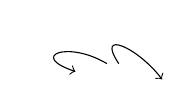
\begin{tikzpicture}
\draw[->] (0,0) .. controls (-.5,.3) and (-1,.1) .. (-.4,-.1);
\draw[->] (.15,0) .. controls (-.15,.45) and (.4,.2) .. (.7,-.2);
\end{tikzpicture}}
% position: lower right operator
\[
\deleted{2\mathrm{id}}\qquad
2\mathrm{id}_{E_1\otimes E_2}
-(\unsure{\pi_{E_1}|\pi'_{E_1}}\otimes\mathrm{id}_{E_2}
+\mathrm{id}_{E_1}\otimes\pi_{E_2})+\pi_{E_1}\otimes\pi_{E_2}
\]
\diagram{\begin{tikzcd}[column sep=large]
x_1\otimes x_2\arrow[r,mapsto]&
\begin{gathered}
2x_1\otimes x_2\unsure{-|+}\pi_1(x_1)\otimes x_2-x_1\otimes\pi_2(\unsure{x_2|x_1})\\
{}+\pi_1(x_1)\otimes\pi_2(x_2)
\end{gathered}
\end{tikzcd}}
% position: bottom left
\[
\overline{x}_1=T_1\psi_1(x_1)-x_1=x_1-\pi_1(x_1)
\]
\[
\pi_1(x_1)=2x_1-T_1\psi_1(x_1)
\]
% position: bottom right cancelled expression
\[
\deleted{\equiv x_1\otimes x_2+(\overline{x}_1\otimes\overline{x}_2)}
\]
\margin{151}

\scanpage{153}
\mspage{476}
% position: upper note 108 1
\(({}^{108}1)\) (6 octobre) Je veux dire que les forces de nature répressive qui ont joué
dans ma vie, semblent prendre surtout, sinon exclusivement, l'une de ces deux
formes spécifiques: enterrement du passé, et mise en avant de mes traits ``\unsure{virils|virils''}
au détriment de mes traits ``féminins''. Je n'entends nullement dire que ces deux
``forces'', de nature répressive l'une et l'autre (c'est à dire, visant à un ``re-\linebreak
foulement'', à un escamotage d'une certaine réalité), soient les seules qui aient
``dominé ma vie''! Ce serait oublier tout l'aspect non égotique de mon être, la
pulsion de connaissance s'exprimant aussi bien au niveau de corps que de \unsure{l'espri|l'esprit}
(Voir à ce sujet notamment ``Mes passions'', section n° 35.)

% position: middle paragraph
Même parmi les forces stucturant le moi, émanation du ``patron'' donc, il en
est au moins une, de nature non répressive par elle-même, bien antérieure aux
forces de répression et dont le rôle dans ma vie a été\quad plus essentiel encore:
c'est l'identification à mon père, qui a été comme ``le coeur paisible et \unsure{puissan|puissant''}
du sentiment de ma propre force. Cette identification n'allait nullement dans le
sens de l'exaltation de certaines valeurs ou qualités (viriles disons) au détri-\linebreak
ment d'autres (``féminines''). Indépendamment des valeurs professées par mon père,
sa personne (jusqu'en 1933, où un basculement a eu lieu en lui (*)), a été em-\linebreak
preinte d'un fort équilibre yin-yang, où l'intuition et la spontanéité n'avaient
pas une moindre part que l'intellect et la volonté.

% position: lower paragraph
Enfin, comme autre ``force'' importante de nature égotique, intimement liée,
elle, aux mécanismes répressifs (ou pour mieux dire, de nature ``répressive''
elle-même), il convient encore de compter la sempiternelle \mbox{v a n i t é}, dont
le rôle a été aussi lourd dans ma vie que dans celle de quiconque. Mais cette
``force''-là est de nature si universelle, tout comme le rôle dominant qu'elle
joue dans la vie de chacun (sous une forme plus ou moins grossière ou subtile),
qu'il n'y a guère lieu de l'inclure expressément, dans un relevé des formes spé-\linebreak
cifiques que prennent chez une personne les forces et mécanismes qui structurent
le moi, et donnent à celui-ci sa physionomie particulière et son assise.

% position: footnote rule
\figure{\begin{tikzpicture}\draw (0,0)--(3,0);\end{tikzpicture}}
% position: footnote
(*) Chose remarquable\inserted{,}ce ``basculement'' chez mon père (agé alors de 43 ans) s'est
fait vers un état \mbox{s u p e r - y i n}, vers une sorte de passivité de pacha, en
étroite connivence avec ma mère, jouant un rôle super-yang. Celle-ci l'a pris en
charge\quad lieu et place de ses enfants.(Ils sont largués aux ``profits et per-\linebreak
tes'', jusqu'en 1939 tout au moins, l'année où sous la pression des événements et
à son corps défendant, elle finit par me reprendre auprès d'elle...) Cette rela-\linebreak
tion de dépendance de mon père et de renversement des rôles yin-yang entre mes
parents, a duré jusqu'à la disparition de mon père en 1942.
% position: left foot short mark
\margin{\unsure{-}}
% position: foot pencil
\margin{152}

\scanpage{154}
% position: top deleted tensor and decomposition
\deleted{\(E_1\otimes E_2\)}
\figure{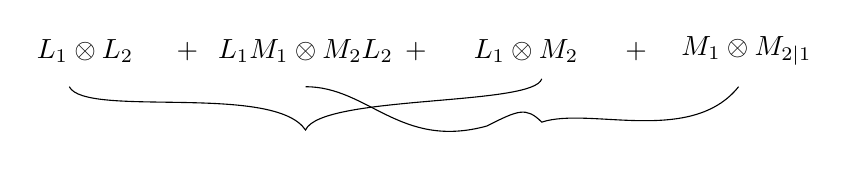
\begin{tikzpicture}[x=1cm,y=1cm]
\node at (0,0) {$L_1\otimes L_2$};
\node at (1.3,0) {$+$};
\node at (2.8,0) {$\unsure{\deleted{L_1}\inserted{M_1}}\otimes\unsure{\deleted{M_2}\inserted{L_2}}$};
\node at (4.2,0) {$+$};
\node at (5.6,0) {$L_1\otimes M_2$};
\node at (7.0,0) {$+$};
\node at (8.4,0) {$M_1\otimes M_{\unsure{2|1}}$};
\draw (-.2,-.45) .. controls (0,-.85) and (2.4,-.4) .. (2.8,-1.0)
 .. controls (3.0,-.55) and (5.7,-.7) .. (5.8,-.35);
\draw (2.8,-.45) .. controls (3.6,-.45) and (4.0,-1.25) .. (5.1,-.95)
 .. controls (5.5,-.75) and (5.6,-.7) .. (5.8,-.9)
 .. controls (6.4,-.7) and (7.7,-1.2) .. (8.3,-.45);
\end{tikzpicture}}
% position: upper diagram
\diagram{\begin{tikzcd}[column sep=large,row sep=large]
E_1\otimes_{0}E_2 \arrow[r,"F_{11}^{!}"] \arrow[dd] \arrow[dr,"\pi"'] \arrow[ddr,bend right=35,dash]
 & E_1\otimes E_2 \arrow[r] & E_1\otimes^{0}E_2 \\
 & L_1\otimes\unsure{L_2|E_2} \arrow[u,"\alpha_1\otimes\alpha_2"'] \arrow[ur,bend right=15,dash,"\deleted{\uline{\unsure{comm.}}}"'] & \\
E_1\otimes\unsure{E_2|\Omega} & M_1\otimes M_2 \arrow[l,"\psi_1\otimes\psi_2"] \arrow[uur] &
\end{tikzcd}}
% reading question: the lower horizontal stroke has a left-pointing thick end; a plain dash is also possible.
% position: right isolated tensor product
\[
(E_1\otimes M_2)\times(M_1\otimes E_2)
\]
% position: short sequence above table
\diagram{\begin{tikzcd}L_1\otimes L_2\arrow[r,dash]&\mathcal O\arrow[r,dash]&\mathcal O\end{tikzcd}}
\[\deleted{\unsure{2|E}}\]
% position: coefficient table
\diagram{\begin{array}{c|cccc}
 & L_1\otimes L_2 & L_1\otimes M_2 & M_1\otimes L_2 & M_1\otimes M_2\\\hline
L_1\otimes L_2 & \chi & \mathrm{id}_{L_1}\otimes\tau_2 & \tau_1\otimes\mathrm{id}_{L_2} & ?\ (\tau_1\otimes\tau_2\ ?)\\[1em]
L_1\otimes M_2 & 0 & 0 & 0 & \uline{?}\ .\tau_1\otimes\mathrm{id}_{M_2}\\[1em]
M_1\otimes L_2 & 0 & 0 & 0 & \uline{?}\ \deleted{\unsure{\tau_2}}\mathrm{id}_{M_1}\otimes\tau_2\\[1em]
M_1\otimes M_{\unsure{1|2}} & 0 & 0 & 0 & \chi
\end{array}}
\figure{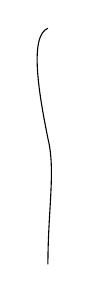
\begin{tikzpicture}\draw (0,0).. controls (-.25,-.1) and (-.1,-.9)..(0,-1.4)..controls (.1,-1.8) and (0,-2.3)..(0,-3);\end{tikzpicture}}
% position: lower prose following table
On \unsure{trouve} que les 2 \unsure{homotopies|contraintes}\deleted{\unsure{compatibilités}} \unsure{comm.}\inserted{sur \(F_{11}\)}
\unsure{sont} \unsure{compatibles}, et \unsure{laissent} une \unsure{indétermination},
qui est un \unsure{hom} de \(M_1\otimes M_2\) en \(L_1\otimes L_2\).
% position: lower isolated formulas
\[
-\qquad E_1\otimes E_2\qquad E_1\otimes E_2
\]
\diagram{$\begin{array}{ll}
\pi'_1=\alpha_1\pi_1\,/\,\omega'_1=\unsure{\varpi_1|\omega_1}\psi_1 & \pi'_1+\bar\omega\\[.6em]
\pi'_2=\alpha_2\pi_2\qquad \unsure{\bar\omega'_2|\varpi'_2}=\omega_2\psi_2 &
\end{array}$}
% position: bottom paragraph
C'est \unsure{normal}, car pour \unsure{l'instant} on n'a \unsure{écrit} \uline{que}
le \unsure{fait} que \unsure{va|on a} \unsure{un} \unsure{iso|de} \unsure{d'extensions|déterminés} - \unsure{et} \unsure{elle}
\unsure{ce|ci} \unsure{sont} \unsure{triviales|faciles}, \unsure{vu|via} \unsure{l'indécision} des choix !
% position: foot pencil
\margin{153}

\scanpage{155}
\mspage{479}
% position: upper continuation paragraph
rant quatre heures je me suis enfoncé dans le sens de ce vécu-là, de ce rêve-pa-\linebreak
rabole, à travers des couches successives de signification de plus en plus brû-\linebreak
lantes, avant d'arriver au coeur du message, à son sens simple et \unsure{evident|évident}.

% position: upper second paragraph
Ce n'a pas été alors le déclic subit d'une compréhension de ``l'intelligen-\linebreak
ce''\inserted{,}ni même comme une lumière subite dans une obscurité ou dans une pénombre.
C'était plutôt comme une vague profonde née en moi et qui soudain déferlait à
travers moi et dans ses vastes eaux m'apportait ce sens qui s'était dérobé
jusque là: que je retrouvais en ce moment un être très cher et très précieux,
que j'avais perdu depuis mon enfance...

% position: middle long paragraph
Ce moment a été vécu comme une \mbox{n a i s s a n c e}, comme un renouvelle-\linebreak
ment profond. Ce sentiment est resté très fort toute cette journée\inserted{,}et encore
dans les jours suivants. Avec le recul de huit ans, ce moment m'apparaît aujour-\linebreak
d'hui encore comme un moment créateur entre tous dans ma vie, et celui d'un tour-\linebreak
nant essentiel dans mon aventure spirituelle. Il a été préparé certes par bien
d'autres ``moments'', dans les jours et dans les mois qui avaient précédé. Le pre-\linebreak
mier précurseur peut-être a été cet ``arrachement salutaire'', plus de dix ans
auparavant, d'une institution où je comptais bien finir mes jours (*). Ces mo-\linebreak
ments antérieurs m'apparaissent un peu comme les ingrédients, ou plutôt comme
les \mbox{m o y e n s} à ma disposition, avec lesquels je pouvais franchir cet au-\linebreak
tre ``seuil'' qui était devant moi sans que je l'aperçoive, qui se situait à un ni-\linebreak
veau plus profond, plus caché que d'autres que j'avais franchis. Tout était réu-\linebreak
ni, depuis quelques jours ou heures, pour que je le franchisse - et je pouvais
le franchir, comme je pouvais ne pas le franchir, jour après jour ma vie durant..

% position: lower paragraph
Et aussi, ce seuil étant bel et bien franchi, la voie s'est trouvée ou-\linebreak
verte vers d'autres franchissements encore, vers d'autres ``éveils'' ou ``réveils'',
dont chacun par nature est aussi un renouvellement, et tant soit peu, une\unsure{:}``nou-\linebreak
velle naissance'', une re-naissance. Il m'est arrivé d'en éluder certains des mois
voire des années durant, pour finir par franchir le pas, m'allégeant au passage
de quelque illusion tenace, qui une vie durant s'était interposée entre moi et
la pleine saveur de ma vie et du monde qui m'entoure. Et sûrement aussi, il en
est que je continue à éluder, au moment encore où j'écris ces lignes...

% position: footnote rule
\figure{\begin{tikzpicture}\draw (0,0)--(3,0);\end{tikzpicture}}
% position: footnote
(*) Voir la note n° 42, de même nom.
% position: foot pencil
\margin{154}

\scanpage{156}
% position: top cancelled calculation
\[\deleted{-\chi(1-\delta\chi)}\]
\[\unsure{\xi|\delta}\]
% position: boxed upper formula
\[
\boxed{\begin{aligned}
&-\chi(1-\delta\chi)x_1\otimes x_2+(1-\delta\chi)[x_1\otimes\pi_2(x_2)+\pi_1(x_1)\otimes x_2)\\
&\hspace{6em}+\delta\pi_1(x_1)\otimes\pi_2(x_2)
\end{aligned}}
\]
% position: text and coefficient values below box
Si \(\chi=2\), on \unsure{peut} prendre \(\delta=1\)

donc
\[
\begin{aligned}
\alpha&=-2(1-2)=2\\
\beta&=\gamma=1-2=-1
\end{aligned}
\]
donc
\[
2x_1\otimes x_2-[(x_1\otimes\pi_2(x_2)+\pi_1(x_1)\otimes x_2)]+\pi_1(x_1)\otimes\pi_2(\unsure{x_2)}
\]
% position: middle cancelled formula
\[\deleted{\pi_i(x_i)=2x_i-T_i\psi(x_i)}\]
% position: middle bar formulas
\[
\begin{aligned}
\pi_i(x_i)&=2x_i-T_i\psi_i(x_i)=2x_i-(x_i+\bar x_i)\\
&&\hspace{9em}\unsure{x_i}-\bar x_i\\
\bar x_i&=.T_i\psi_i(x_i)-x_i\qquad\deleted{=\unsure{x}}\\[.7em]
x_i+\bar x_i&=T_i\psi_i(x_i)
\end{aligned}
\]
% position: lower tensor expansion
\[
\begin{aligned}
&2x_1\otimes x_2-[(\uline{x_1\otimes(x_2}-\bar x_2)+(x_1-\uline{\bar x_1)\otimes x_2})]
+\uline{(x_1-\bar x_1)\otimes(x_2}-\unsure{\overline{\overline{x_2}})|\bar x_2)}\\
&\qquad=x_1\otimes x_2+\bar x_1\otimes\bar x_2\qquad\text{o.K.}
\end{aligned}
\]
% position: lower left separator
\figure{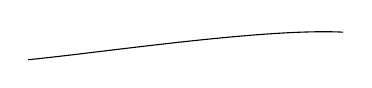
\begin{tikzpicture}\draw (0,0)..controls (1,.1) and (3,.4)..(4,.35);\end{tikzpicture}}
% position: lower unfinished bar expression
\[
\overline{\unsure{X_i|x_i}}=x_i-\pi_i(x_i)=\bigl\{
\]
% position: bottom cancelled tensor continuation
\[
x_1\otimes x_2+\deleted{(\unsure{x_1}-\unsure{\pi_1(x_1)}}
\]
% position: bottom coefficient equations
\[
\begin{gathered}
-\chi(1-\delta\chi)\overset{?}{=}\chi\\[.8em]
-1+\delta\chi=1\qquad\boxed{\delta\chi=2}\\
\unsure{:|-}
\end{gathered}
\]
% position: foot pencil
\margin{155}

\scanpage{157}
\mspage{486}
% position: upper continuation paragraph
très fort auprès des femmes dont j'ai été amant par la suite, en réveillant en
l'amante des pulsions masculines, qui durant toute sa vie avaient été soigneu-\linebreak
semant refoulées, et n'avaient trouvé à s'exprimer jusque là qu'``à la sauvette''
comme des sortes de bavures, indignes de figurer dans le vécu amoureux conscient

% position: upper long paragraph
Le vécu amoureux inconscient est riche de pulsions archétypes, dont une \unsure{de|des}
plus puissantes est celle du retour à la Mère, du retour dans le giron originel.
Un tel archétype est présent dans les couches profondes de l'expérience amoureu-\linebreak
se, chez l'homme et aussi chez la femme. En la femme, les résistances à la sa-\linebreak
tisfaction d'une telle pulsion dans le vécu amoureux du couple sont plus fortes
encore que chez l'homme, où elle se heurte à un tabou-clef, et non à deux comme
chez elle. Chez l'un comme chez l'autre, la satisfaction de ces pulsions \unsure{-}dans
le vécu commun reste souvent plus ou moins symbolique et surtout,
dérobé à la conscience. Quand un tel archétype et ce vécu remontent des couches
profondes jusqu'à la lumière du jour, dans le champ du regard conscient, ce
vécu aussitôt se transforme, il acquiert une dimension nouvelle. En même temps
se libèrent des énergies considérables, précédemment comprimées par les mécanis-\linebreak
mes répressifs, ou liées par les tâches de répression. L'effet est celui d'une
\mbox{l i b é r a t i o n} immédiate de la pulsion érotique, se manifestant par une
intensité renouvelée et par une plénitude nouvelle dans l'expérience amoureuse.

% position: lower long paragraph
Par ce qui précède, il apparaîtra déjà, sûrement, que cette acceptation
nouvelle de ma propre personne est allée de pair avec une acceptation d'autrui.
L'un et l'autre sont indissolublement liés. Il est entendu qu'il s'agit ici
d' ``acceptation'' dans le plein sens du terme, qui ne signifie nullement une
\mbox{t o l é r a n c e} (souvent aigre-douce) vis-à-vis de tels et tels ``travers'' ou
``défauts'', ressentis comme un mal hélas inévitable, pour lequel on est bien
obligé de ``faire avec''. Dans une telle attitude, je sens surtout une résignation,
pour ne pas dire une abdication, et sûrement pas une source de joie, ni un élan
de prise de connaissance d'une chose digne d'être connue: la profondeur préssen-\linebreak
tie\inserted{,}inconnue, derrière la plate surface de tels ``défauts'' ou ``travers'' qu'on
veut bien tolérer...

% position: bottom paragraph
Qu'il s'agisse ici d'une acceptation joyeuse, créatrice, ne signifie nulle-\linebreak
ment pour autant que cette acceptation soit totale-hier déjà j'ai constaté qu'il
n'en était rien. Un lecteur attentif l'aura déjà constaté par lui-même plus d'une
fois au cours de Récoltes et Semailles, comme il m'est arrivé de m'en
% position: left foot short mark
\margin{\unsure{-}}
% position: foot pencil
\margin{156}

\scanpage{158}
% position: upper cancelled fragments
\[
\deleted{\alpha u_1\otimes x_2+}\qquad
\deleted{\alpha\unsure{u_1}+\chi\gamma}
\]
\figure{
\begin{tikzpicture}\fill[gray!55] (0,.7)--(.65,.14)--(.48,0)--cycle;\draw (0,.7)--(.6,.13);\draw (.28,.38)--(.57,.07);\draw (.37,.3)--(.52,-.03);\end{tikzpicture}}
% position: upper coefficient expression
\[
\begin{aligned}
&(\alpha+\chi\gamma)u_1\otimes x_2+(\beta\deleted{\unsure{x_1|\chi}}+\delta\chi)u_1\otimes\pi_2(x_2)\\
&\hspace{17em}\Vert\\
&\hspace{15em}u_1\otimes\pi_2(x_2)
\end{aligned}
\]
% position: upper vanishing identity and quantifiers
\[
(\alpha+\chi\gamma)u_1\otimes x_2+(\beta+\delta\chi-1)u_1\otimes\pi_2(x_2)=0
\]
\[
\forall u_1\in L_1,\quad x_2\unsure{\in|+}E_2
\]
Si \(x_2=u_2\) on \unsure{trouve}
\margin{\unsure{et.|eff.}}
\[
(\alpha+\chi\gamma\deleted{+})+\chi(\beta+\delta\chi-1)=0
\]
% position: middle tensor factor identity
\[
u_1\otimes\uline{[(\alpha+\chi\gamma)x_2+(\beta+\delta\chi-1)\unsure{\pi_2}(x_2)]}=0
\]
Donc sur \(\unsure{L'_2|L_2^1}\) \unsure{on a}.
\[
(\alpha+\chi\gamma)\mathrm{id}=0
\]
% position: middle coefficient consequences
donc
\[
\begin{aligned}
\alpha+\chi\gamma&=0\\
\alpha&=-\chi\gamma
\end{aligned}
\]
donc \unsure{aussi}
\[
\alpha=-\chi\beta\qquad\text{\unsure{et|en}}\quad\uline{\beta=\gamma}
\]
% position: lower cancelled coefficient
\[\deleted{\beta+\delta}\]
% position: lower tensor expression
\[
\begin{aligned}
-\chi\beta x_1\otimes x_2+\beta(x_1\otimes\pi_2(x_2)+\pi_1(x_1)\otimes x_2)+\delta\pi_1(x_1)\\
\hspace{25em}\otimes\pi_2(\unsure{x_2)}
\end{aligned}
\]
% position: lower cancellation and remaining condition
il reste \unsure{en}
\[
\deleted{\unsure{\pi_2 b}\unsure{-|\leftarrow}\unsure{L_1\oplus}\unsure{x}}
\]
\[
(\beta+\delta\chi-1)\pi_2(x_2)=0
\]
% position: bottom boxed condition and right continuation
\[
\boxed{\beta+\delta\chi=1}\qquad
\begin{aligned}
\beta&=1-\delta\chi\ .\\
\alpha&=-\chi\beta=\\
&\deleted{-\chi+\chi^2}
\end{aligned}
\]
% position: foot pencil
\margin{157}
% position: bottom left marginal coefficients
\margin{\(\begin{aligned}
\beta&=\unsure{\deleted{\beta}\inserted{\gamma}}=1-\delta\chi\\
\alpha&=-\chi(1-\delta\chi)
\end{aligned}\)}

\scanpage{159}
\mspage{487}
% position: upper continuation paragraph
rendre compte en passant, quand je me voyais confronté à nouveau à ce sempiter-\linebreak
nel mécanisme en moi de \mbox{r e j e t} de tout ce qui se présente sous une appa-\linebreak
rence déplaisante, chez autrui ou chez moi-même. (Mais quand il d'agit de soi-\linebreak
même, ce mécanisme le plus souvent a comme effet de ne pas même prendre connais-\linebreak
sance de la chose déplaisante en question...)

% position: middle long paragraph
L'acceptation dont je parle prend racine dans un \mbox{i n t é r ê t} pour
cette chose qu'on ``accepte'', chez soi-même ou chez autrui. Alors que l'accepta-\linebreak
tion est par elle-même une disposition intérieure de caractère typiquement ``yin''\unsure{;}
cette connotation d'``intérêt'' qu'elle prend chez moi est de nature ``yang'' - \unsure{c'es|c'est}
le ``yang dans le yin'', dans la délicate dialectique chinoise de l'entrelacement
à l'infini du yin et du yang... J'allais me hasarder à dire, un peu dans la fou-\linebreak
lée\inserted{,}qu'il y avait une identité pure et simple entre l'acceptation (la vraie!)
et cet intérêt, cette curiosité. Pourtant, en posant un peu sur la chose, je me
rends compte qu'il y a bien aussi une autre façon d'accepter, de nature, elle,
plus totalement yin que celle qui m'est surtout coutumière. C'est comme un
\mbox{a c c u e i l} de la chose acceptée, et non un élan vers elle pour la sonder.
(Cette nuance d'accueil m'apparaît du coup comme le ``\mbox{y i n}\quad d ans le yin'',
nous y voilà!) L'élan de l'intérêt, et l'attitude d'accueil, peuvent l'une com-\linebreak
me l'autre former la note de fond de l'acceptation d'autrui ou de soi. La chose
commune aux deux est la \mbox{s y m p a t h i e}. C'est là aussi une des formes de
l' \mbox{a m o u r}. S'il y a quelque identité profonde à cerner ici, ce serait
donc par la constatation que \mbox{l' a c c e p t a t i o n\quad e s t\quad u n e}
\mbox{f o r m e\quad d e\quad l' a m o u r}. Amour de soi, amour de l'autre, l'un et l'au-\linebreak
tre indissolublement liés...

% position: lower long paragraph
Sauf en de rares instants, mon intérêt est plus intensément impliqué quand
il s'agit de ma propre personne, que de celle d'autrui. C'est cet intérêt passio-\linebreak
né pour ma personne qui a animé les longues périodes de méditation, au cours
de ces huit dernières années. Il est vrai que c'est bien la connaissance de soi
qui est au coeur de la connaissance d'autrui et du monde, et non l'inverse - et
je sens que c'est bien vers le coeur des choses, vers le plus essentiel, que
m'a porté et me porte encore ma nouvelle passion, la méditation. L'intérêt pour
autrui est apparu de façon plus parcellaire et plus réticente au cours de ces
années, tout comme l'acceptation qui en découle. Une des façons dont elle s'est
manifestée concrètement, c'est par une propension moins grande à parler quand je
suis en compagnie, et par une attitude d'écoute. La plus grande partie de ma vie,
cette capacité d'écoute m'avait presque entièrement fait défaut. Encore après
le grand tournant des retrouvailles, il m'a fallu constater bien souvent encore
% position: left foot short mark
\margin{\unsure{-}}
% position: foot pencil
\margin{158}

\scanpage{160}
% position: top two sequences
\diagram{\begin{tikzcd}
0\arrow[r,dash]&\unsure{\deleted{E_1}\inserted{L_1}}\arrow[r,dash]&E_1\arrow[r,dash]&\unsure{L'_1}\arrow[r,dash]&0\\
0\arrow[r,dash]&L_2^{\unsure{4|+}}\arrow[r,dash]&E_2\arrow[r,dash]&L'_2\arrow[r,dash]&0
\end{tikzcd}}
% position: upper right note
\margin{\(L_1,L'_1\) \unsure{qcq} \unsure{ici.}\par
\unsure{non.} Mais \unsure{suppos.} \(L'_1,L'_2\)
loc. libres de rang fini}
% position: left mark by middle sequence
\margin{\unsure{\(\longrightarrow\)|-}}
% position: middle sequence
\diagram{\begin{tikzcd}
0\arrow[r,dash]&L_1^{\unsure{4|+}}\otimes L_2\arrow[r,dash]&E_1\wedge E_2\arrow[r,dash]&L'_1\otimes L'_2\arrow[r,dash]&0
\end{tikzcd}}
% position: dual sequence
\diagram{\begin{tikzcd}
0&L_1^\vee\otimes L_2^\vee\arrow[l]&E_1^\vee\wedge E_2^\vee\arrow[l]&L_1'{}^\vee\otimes L_2'{}^\vee\arrow[l]&0\arrow[l]
\end{tikzcd}}
\figure{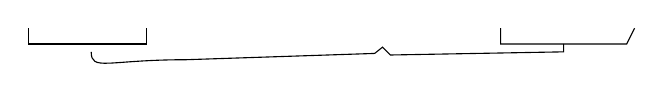
\begin{tikzpicture}
\draw (0,.2)--(0,0)--(1.5,0)--(1.5,.2);
\draw (6,.2)--(6,0)--(7.6,0)--(7.7,.2);
\draw (.8,-.1)..controls (.8,-.35) and (1,-.2)..(2,-.2)--(4.4,-.12)--(4.5,-.04)--(4.6,-.14)--(6.8,-.1)--(6.8,0);
\end{tikzpicture}}
% position: middle assertion
Je dis que
\[
E_1^\vee\wedge E_2^\vee\simeq(E_1\wedge E_2)^\vee
\]
% position: Hom expression
\[
\operatorname{Hom}(L'_1,\unsure{k|\mathcal O})\otimes\operatorname{Hom}(L'_2,\unsure{k|\mathcal O})
\simeq\operatorname{Hom}(L'_1\otimes L'_2,\unsure{k|\mathcal O})
\]
% position: lower initial pairing
\[
\unsure{f_1}\otimes f_2+\bar f_1\otimes\bar f_2,\quad x_1\otimes x_2
\]
% position: lower left diagram
\diagram{\begin{tikzcd}[row sep=small,column sep=large]
\unsure{A|\mathcal A}_1\otimes\unsure{A|\mathcal A}_2\arrow[dd,Rightarrow]\arrow[dr] &\\
&\unsure{A|\mathcal A}_1\otimes\unsure{A|\mathcal A}_2\\
L_1\otimes L_2\arrow[ur,"\begin{gathered}\pi_1\otimes\mathrm{id}\\\mathrm{id}\otimes\pi_2\end{gathered}"']&
\end{tikzcd}}
% position: lower middle trace products
\[
\begin{aligned}
&(\operatorname{Tr}_1(f_1)-f_1)\otimes(\operatorname{Tr}_2(\unsure{f_2})-\unsure{f|f_2})\\
&(\pi'_1(f_1)-f_1)(\pi_2(\unsure{f_2})-\unsure{f|f_2})
\end{aligned}
\]
% position: isolated f signs
\[
\unsure{f_4|\deleted{f_4}}\qquad\unsure{f_2|\deleted{f_2}}\qquad f_1
\]
% position: lower left pi fragments
\margin{\(\pi_1(x_1)-\)}
% position: lower sigma expressions
\[
\deleted{\sigma=\unsure{\pi}}\qquad\sigma(x)=\operatorname{Tr}(x).1-x
\]
\[
\sigma\equiv T\otimes\unsure{\ell|e}-\mathrm{id}
\]
% position: right sloping marginal formulas
\margin{\(\begin{gathered}
2x-\psi(x)T\\
\uline{x-\psi(x)T}\\
=-\sigma(x)
\end{gathered}\)}
% position: lower left second pi fragment
\margin{\(\pi_1(x_1)\)}
% position: lower right isolated trace expression
\margin{\(u_1\otimes\uline{\operatorname{Tr}(x_2)}=\unsure{i|1}\)}
% position: lower tensor maps
\[
\begin{aligned}
\unsure{u_1|x_1}\otimes x_2&\longmapsto\deleted{\unsure{\pi_1}(\unsure{x_1|u_1})\otimes x}\quad u_1\otimes\pi_2(x_2)\\
x_1\otimes u_2&\unsure{\vdash|\longmapsto}\pi_1(x_1)\otimes u_2
\end{aligned}
\]
% position: bottom boxed tensor expression
\[
\boxed{x_1\otimes x_2+\pi'_1(x_1)\otimes\pi'_2(x_2)}
\]
% position: bottom right marginal computation
\margin{\(\unsure{(\chi-1)x|(\chi-1)^x}\)
\figure{\begin{tikzpicture}\draw[->] (.8,.5)..controls (.9,.05) and (.15,.3)..(0,0);\end{tikzpicture}}
\(\pi_2(x)=\unsure{x|\bar x}+\pi'_2(x)\)
\(\left\{\begin{array}{l}
\text{Si }x\in L_2,\ \text{\unsure{on}.}\\
\pi'_2(\unsure{x})=\unsure{x}
\end{array}\right.\)}
% position: foot pencil
\margin{159}

\scanpage{161}
\mspage{489}
% position: top continuation
son bon vouloir - par où en somme il nous ``tient'', et (mine de rien) nous manoeu-\linebreak
vre à sa guise...

% position: main paragraph
En bonne logique, l'acceptation d'autrui devrait bien impliquer aussi
l'acceptation de sa façon de voir les choses, qu'elles nous paraissent erronées
ou non, et même lorsqu'il s'agit de sa façon de voir notre propre et précieuse
personne (y inclus nos propres façons de voir...). C'est surtout là pourtant que
le bat blesse - c'est \mbox{l à} le point névralgique dans l'acceptation d'autrui,
et nullement dans l'acceptation de ``défauts'' courants plus ou moins gênants qui
n'impliquent pas directement notre personne. Bien souvent d'ailleurs, si nous \unsure{re|reje-}\linebreak
tons tels ``défauts'' en autrui, c'est surtout parce que par eux nous nous sentons
mis en cause directement, du seul fait d'être confronté à des façons d'être
qui nous paraissent (à tort ou à raison encore) à l'opposé des nôtres. En d'au-\linebreak
tres mots, c'est une \mbox{i n s é c u r i t é} en nous, se manifestant par les
réactions (plus ou moins apparentes ou cachées) de la vanité, qui est le grand
obstacle, s'opposant à notre acceptation d'autrui. Mais cette insécurité pro-\linebreak
fondément enracinée, compensée par les mouvements de la vanité, m'apparaît com-\linebreak
me \unsure{insissolublement|indissolublement} liée à la non-acceptation de nous-même, elle en est comme l'\unsure{o|om-}\linebreak
bre inséparable.

% position: concluding upper paragraph
Ainsi, c'est la pleine acceptation de soi qui apparaît ici comme la clef
qui nous ouvre à l'acceptation d'autrui. Et ce lien qui vient de m'apparaître
ici, rejoint un autre lien profond, que je connais depuis longtemps, depuis tou-\linebreak
jours peut-être: que l'amour de soi est le coeur, paisible et fort, de l'amour
de l'autre.

% position: lower note 111
\(({}^{111})\) (13 octobre) Hier je n'ai pas continué à écrire les notes. Au lieu de cela\unsure{.|,}
je me suis amusé à repasser en revue un certain nombre de ``couples'' yin-yang.\unsure{\inserted{:}}
Commençant par ceux qui me passaient par la tête, un peu au-bonheur-la-chance,
je me suis ensuite piqué au jeu, et ai terminé par une sorte de ``recensement'' de
tous ceux sur lesquels j'arrivais à mettre la main. J'avais commencé parce que
je m'étais dit que pas mal de ce que j'avais écrit dernièrement risquait fort de
passer entièrement ``par dessus la tête'' d'un lecteur qui ne serait déjà tant \unsure{soi|soit}
peu familier du double aspect yin-yang des choses. Il ne serait peut-être pas
inutile de prendre la peine de donner au moins quelques exemples frappants de
tels couples, en plus de ceux qui s'étaient introduits par la bande ces derniers
% position: left foot mark
\margin{\unsure{-}}
% position: foot pencil
\margin{160}

\scanpage{162}
% position: top definition
\[
x\longmapsto\pi'(x)=\pi(x)-(\chi-1)x
\]
% position: top right sequence
\margin{\diagram{\begin{tikzcd}0\arrow[r,dash]&L\arrow[r,dash]&E\arrow[r,dash]&L'\arrow[r,dash]&0\end{tikzcd}}}
% position: upper deleted fragment and E map
\deleted{\unsure{pour}}
\diagram{\begin{tikzcd}E\arrow[r,dash]&E\end{tikzcd}}
% position: upper restriction conditions
\[
\deleted{\unsure{\pi'(L')}}\quad
\left\{\begin{array}{l}
\pi'|L)=\deleted{\unsure{\chi}}\ \mathrm{id}_L\quad\Longleftrightarrow\quad\pi|L=\chi\,\mathrm{id}_L\\
\pi'|E/L=L')=-(\chi-1)\mathrm{id}_{L'}
\end{array}\right.
\]
\[
\Longleftrightarrow\quad\pi:E\unsure{\longrightarrow|-}L
\]
% position: left deleted pi fragment
\deleted{\(\unsure{\pi'(x)}\)}
% position: middle tensor calculation
\[
\unsure{u_1|x_1}\otimes x_2+\underbrace{\pi'_1(x_1)}_{u_1}\otimes\pi'_2(x_2)
=u_1\otimes(\underbrace{x_2+\pi'_2(\unsure{x_2})}_{\displaystyle x_2+\pi_2(x_2)-(\chi-1)x_2}
\]
\[
=\uline{(\unsure{2}-\chi)x_2+\pi_2(\unsure{x_2})}
\]
% position: middle left paired diagrams
\diagram{\begin{tikzcd}[row sep=large]
L_1\arrow[r,phantom,"\subset"]&E_1\arrow[l,bend right=35,"\pi_1\quad\text{\unsure{\(\chi\)-triv.}}"']\\
L_2&E_2\arrow[l]\arrow[l,bend left=35,"\pi_2"]
\end{tikzcd}}
\[\Longrightarrow\]
% position: middle right factorization diagram
\diagram{\begin{tikzcd}[column sep=small,row sep=small]
E_1\otimes E_2\arrow[rr,"?",very thick]\arrow[dr,bend right=10]\arrow[dd]
&&E_1\otimes\unsure{E_2}\arrow[dd]\\
&E\arrow[ur]&\\
E_1\otimes\unsure{E_2|L_2}\mathop{\oplus}\limits_{L_1\otimes L_2}L_1\otimes\unsure{E_1|E_2}
\arrow[rr,"{\pi_1,\pi_2}"']\arrow[dr]&&\unsure{L'_1|L_1}\otimes L_2\arrow[dl,dash]\\
&L'_1\otimes L'_2&
\end{tikzcd}}
% position: lower three-row diagram
\diagram{\begin{tikzcd}[row sep=large,column sep=large]
\unsure{0}\arrow[r,dash]&E_1\otimes_0 E_2\arrow[r,dash]\arrow[d,"\operatorname{Tr}"]
&E_1\otimes E_2\arrow[r,dash]\arrow[d,dash]&L'_1\otimes L'_2\arrow[r,dash]\arrow[d,Rightarrow]&0\\
\unsure{0}\arrow[r,dash]&\unsure{\deleted{E_1}\inserted{L_1}}\otimes L_2\arrow[r,dash]\arrow[d,"\text{\unsure{inc. can.}}"]
&E\arrow[r,very thick]\arrow[d,"?"]&L'_1\otimes L'_2\arrow[r,dash]\arrow[d,"{\chi\,\mathrm{id}}"]&0\\
0\arrow[r,dash]&E_1\otimes_0 E_2\arrow[r,dash]&E_1\otimes E_2\arrow[r,dash]&L'_1\otimes L'_2\arrow[r,dash]&{}
\end{tikzcd}}
% position: bottom deleted fragments
\[
\deleted{\unsure{x_1}\quad\pi_1}\qquad\deleted{\alpha+}
\]
% position: bottom paired expressions
\[
\unsure{x_1|a_1}\quad\pi_1(x_1)\qquad \unsure{x_2|a_2},\pi_2(x_2)
\]
% position: bottom tensor polynomial
\[
\alpha\ x_1\otimes x_2+\beta\,\unsure{x_1|x_2}\otimes\pi_2(x_2)
+\gamma_{\unsure{2|.}}\,\pi_1(x_1)\otimes x_2+\delta\,\pi_{\unsure{1|2}}(\unsure{x_1})\otimes\pi_2(x_2)
\]
% position: foot pencil
\margin{161}

\scanpage{163}
\mspage{488}
% position: upper continuation paragraph
que j'avais parlé à contre temps, faute d'écoute et de discernement, avant que
cette propension invétérée commence à me passer. Si elle est devenue beaucoup
moins envahissante, et qu'elle a même quasiment disparue, ce n'est nullement \unsure{com|com-}\linebreak
me résultat de quelque discipline que je me serais imposé\inserted{\unsure{e}} (style: tu n'ouvriras
le bec que si...). C'est simplement parce que l'envie m'a passé de parler, en \unsure{de|des}
moments où je sens bien que c'est inutile, que cela n'apporte rien à autrui ni
à moi - rien du moins qui ait une valeur à mes yeux. Si à présent j'arrive sou-\linebreak
vent à sentir de telles choses, c'est sans doute que je suis devenu plus atten-\linebreak
tif. Cela aussi n'est pas venu comme fruit d'une discipline (``tu vas faire
gaffe d'ouvrir grandes tes oreilles quand...''), mais je ne saurais dire comment.
En tous cas, je m'en sens mieux, la vie est d'autant plus intéressante (et sur-\linebreak
tout moins bruyante!). Et les autres aussi s'en sentent mieux...

% position: lower paragraph
Je crois que j'ai commencé à vraiment moins parler, à partir du moment
où à disparu (autant dire) cette force en moi qui me pousse à toujours vouloir
rectifier ce qui m'apparaît (à tort ou à raison) comme des ``erreurs'' chez au-\linebreak
trui - comme s'il n'était pas suffisant que je décèle et rectifie les miennes!
C'est la force aussi qui me poussait (et parfois encore me pousse) à vouloir
à toute fin convaincre autrui de ceci ou de celà, au lieu de regarder simplement
pourquoi untel préfère mordicus croire ceci plutôt que cela (qui me paraît ``ça'',
et dont je voudrais bien le convaincre!); ou pourquoi je tiens tellement à ce
\unsure{qu'il} croie cela, plutôt que ceci. Cette force quasiment universelle en nous,
qui nous pousse constamment à chercher dans l'approbation d'autrui (et ne fut-ce
qu'un seul...) la confirmation du bien-fondé de ce que nous tenons pour vrai -
cette force profondément enracinée dans l'égo a fini, je crois, par lâcher pri-\linebreak
se en moi. Cela a été un grand soulagement, la fin d'une dispersion d'énergie
faramineuse. C'est quand j'ai fini par me rendre compte, il y a deux ans, de la
portée de cette force dans ma vie, de sa nature, et de d'extraordinaire disper-\linebreak
sion d'énergie qu'elle représentait, qu'elle s'est trouvée désamorcée - et que
je me suis trouvé allégé du coup ``d'un poids de cent tonnes''. Prendre connais-\linebreak
sance sans réticence de d'écho qu'autrui nous renvoie de notre personne, sans
être lié par un désir ou ``besoin'' (si caché soit-il) d'approbation ou de confir-\linebreak
mation - c'est cela vraiment, être ``libre de lui''. C'est un tel besoin ou désir
qui constitue véritablement le ``crochet'', discret et d'une solidité à toute
épreuve, par où le conflit peut ``accrocher'' en nous, et par où nous sommes (que
nous le voulions ou le reconnaissions, ou non) sous la dépendance d'autrui, de
% position: left lower mark
\margin{\unsure{-}}
% position: foot pencil
\margin{162}

\scanpage{164}
% position: upper left table
\(\pi'_i\)
\diagram{\(\begin{array}{c|c|c|}
&L_i,&M_i\\\hline
L_i&\chi&\tau_i\\\hline
M_i&0&0\\\hline
\end{array}\)}
\margin{\(\unsure{\prime}\)}
% position: upper middle table
\(\unsure{\varpi'_i|\bar\pi'_i}\)
\figure{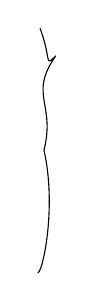
\begin{tikzpicture}
\draw (0,3.1)..controls (.15,2.7) and (.05,2.6)..(.2,2.75)..controls (-.15,2.25) and (.2,2.15)..(.05,1.55)..controls (.22,.8) and (.02,-.05)..(-.03,0);
\end{tikzpicture}}
\diagram{\(\begin{array}{c|c|c}
&L_i&M_i\\\hline
L_i&0&-\tau_i\\\hline
M_i&0&\chi
\end{array}\)}
% position: upper right isolated tensors
\margin{\(\ell_1\otimes m_2\)\par
\((\deleted{\unsure{\ell_1+m_1}}\)}
% position: middle deleted operator
\[
\deleted{\pi'_1\otimes\mathrm{id}_{E_2}+\mathrm{id}_{E_1}\otimes}
\]
% position: middle left empty ruled frame
\figure{\begin{tikzpicture}
\draw (0,2.1)..controls (2,2.3) and (3.1,2.5)..(4.3,2.55);
\draw (.32,2.55)..controls (.3,1.6) and (.55,.7)..(.4,0);
\draw (.36,2.55)--(.36,.55)..controls (.48,.8) and (.45,1)..(.4,1.2);
\end{tikzpicture}}
% position: middle right coefficient table
\diagram{\(\begin{array}{c|ccc}
1&\unsure{\deleted{\mathrm{id}}\inserted{1}}&1&1\\\hline
\pi'_1&\chi&\chi&\tau_1\otimes\mathrm{id}_{L_2}\\[1ex]
\pi'_2&\chi&\mathrm{id}_{L_1}\otimes\tau_2&\chi\\[1ex]
\pi'_1\otimes\pi'_2&\chi^2&\chi\,\mathrm{id}_{L_1}\otimes\tau_2&\chi\tau_1\otimes\mathrm{id}_{L_2}
\end{array}\)}
% position: lower left operator
\[
\alpha+\beta_1\pi'_1+\beta_2\pi'_2+\gamma\pi'_1\otimes\pi'_2
\]
% position: lower left deleted formula
\[
\deleted{\alpha\pi'_1+\beta\pi'}
\]
% position: lower central boxed condition
\[
\deleted{\unsure{\chi}}\quad\boxed{\alpha+(\beta_1+\beta_2)\chi+\gamma\chi^2=\chi}
\]
% position: lower central calculation and bracket
\[
\alpha+\beta_1\chi+
\underbrace{\unsure{\beta_2}\,\mathrm{id}\otimes\tau_2+\gamma\chi\,\mathrm{id}\otimes\tau_2}_{(\beta_2+\gamma\chi)\mathrm{id}\otimes\tau_2}
=\mathrm{id}_{L_1}\otimes\tau_2
\]
% position: bottom left boxed conditions
\[
\boxed{\begin{gathered}
\alpha+\beta_1\chi=0\\
\beta_2+\gamma\chi=1
\end{gathered}}
\]
% position: bottom right marginal expansion
\margin{i.e.\quad\(\begin{gathered}
\mathrm{id}_{L_1}\otimes(\inserted{\alpha+}\unsure{\beta_1}\chi\,\mathrm{id}_{M_2}\\
+(\beta_2+\gamma\chi)\tau_2)=\\
\mathrm{id}\otimes\tau_2
\end{gathered}\)}
% position: foot pencil
\margin{163}

\scanpage{165}
\mspage{477}
% position: note 1082 upper paragraph
\(({}^{108}2)\) (6 octobre) Dans ce ``déployement de force'' il n'y a nulle intention
``agressive'' au sens courant du terme, consciente ni inconsciente, seulement un
désir inconscient d'impressionner, de forcer l'estime. Il est vrai que ce terme
``forcer l'estime'' qui me revient spontanément, porte déjà une connotation de
\mbox{c o n t r a i n t e}, voisine de celle ``d'agression''. Cette intention inconscien-\linebreak
te de contrainte, perçue au niveau inconscient également, doit souvent être \unsure{vécue}
comme une sorte d'agression (alors même que ce vécu reste occulté, tout comme \unsure{les}
réactions antagonistes qu'il déclenche). En même temps, il doit se faire souvent
l'amalgame de ce vécu avec des vécus analogues, remontant à l'enfance, avec le
père comme protagoniste, et où celui-ci apparaît comme le principal détenteur
d'autorité répressive, voire comme un rival écrasant, envié et détesté.

% position: middle paragraph
Même sans un tel amalgame, et indépendamment aussi de toute perception \unsure{chez}
autrui d'une intention de ``contrainte'' en moi, il doit y avoir souvent la per-\linebreak
ception d'un fort \mbox{d é s é q u i l i b r e}, d'une disharmonie foncière, dans
ce ``déployement de force'' exclusivement yang (dans son esprit et intention, au
moins). Cette démesure est néfaste au principal intéressé, savoir moi-même, et
à la limite bel et bien ``dangereux'' pour sa survie physique même (comme des inci-\linebreak
dents-santé de ces dernières années me l'ont bien montré! ). C'est cela sans dou-\linebreak
te qui a été en filigrane dans ma pensée, quand j'écrivais qu' ``un tel \unsure{déployemer|déployement}
de force'' était ressenti ``en tout cas comme dangereux'' - dangereux ``par nature'',
un exemple donc à surtout ne pas suivre...! Un tel ressenti est sûrement suffi-\linebreak
sant pour susciter des ``réactions de défense'', en l'absence même de toute agres-\linebreak
sion ou intention d'agresser.

% position: lower paragraph
Il est vrai que de telles relations d'ambiguité se sont reproduites après
1976, avec certains de mes élèves notamment, en des moments où tout investisse-\linebreak
ment mathématique était absent, et où il n'y avait aucun ``dépoyement de force''
apparent dans ma vie. Il est vrai aussi que les `` déployements'' en question du
\mbox{p a s s é} ont créé une \mbox{r é p u t a t i o n}, qui continue à me coller à la
peau, surtout dans ma vie professionelle, et qui dans une certaine mesure se\inserted{\unsure{,}}
substitue à la perception de celui que je suis \mbox{d a n s\quad l e\quad p r é s e n t}.
De plus, j'ai acquis dans le commerce de certains thèmes mathématiques une aisan-\linebreak
ce telle que, même en dehors de mes périodes mathématiques et ma réputation ai-\linebreak
dant, cette aisance ou maîtrise naturelle peuvent avoir déjà l'effet du ``déploye-\linebreak
ment de force'', sur des élèves peu motivés, et me faire ressentir par eux (en
dépit de certains traits avenants voire rassurants) comme une sorte de Superman
(un peu Superpère sur les bords!).
% position: left lower mark
\margin{\unsure{-}}
% position: right foot pencil rotated
\margin{164}

\scanpage{166}
% position: top sentence
Pour définir un hom \(F\), il faut définir
% position: large central diagram
\diagram{\begin{tikzcd}[column sep=large,row sep=large]
&(E_1\otimes L_2)\unsure{\oplus}(L_1\otimes E_2)=\Sigma
\arrow[dl,"{\mathrm{id}_1\otimes\alpha_2,\alpha_1\otimes\mathrm{id}_2}"']
\arrow[dr,"{\pi_1\otimes\mathrm{id}_{\unsure{L_2|2}},\mathrm{id}_1\otimes\pi_2}"]&\\
E_1\otimes E_2\arrow[dd,"F_{11}"',"\unsure{\times}"{description,pos=0.04}]\arrow[ddrr,"F_{12}" near end]
&&L_1\otimes L_2\arrow[ddll,"F_{21}" near start]\arrow[dd,"F_{22}"]\\
&&\\
E_1\otimes\unsure{\deleted{M_2}\inserted{E_2}}\arrow[dr,"{\mathrm{id}_1\otimes\psi_2,\psi_1\otimes\mathrm{id}_2}"']
&&M_1\otimes M_2\arrow[dl,"{\varpi_1\otimes\mathrm{id}_{\unsure{1|2}},\mathrm{id}_1\otimes\varpi_2}"]\\
&(E_1\otimes M_2)\times(M_1\otimes E_2)=\Pi&
\end{tikzcd}}
% position: right note beside diagram
\margin{\unsure{ces} 4 \unsure{carrés} commu-\linebreak\unsure{tatifs}}
% position: prose below large diagram first condition
Si on veut que \(F\) induise \deleted{l'identité}
\inserted{un hom d'\unsure{extensions}, donc}
\diagram{\begin{tikzcd}L_1\otimes L_2\arrow[r,dash]&L_1\otimes L_2\end{tikzcd}},
il \unsure{f. et s.}
\deleted{\unsure{voir}} que \(\boxed{F_{22}=0}\),
\unsure{si} on veut \inserted{de plus} que \(\unsure{S_0|F}\) induise l'identité sur \(L_1\otimes L_2\),
il \unsure{f. et s.} que \(\boxed{F_{21}=\alpha_1\otimes\alpha_2}\),
si on veut que \(\unsure{F'|F}\) induise l'identité
sur \(M_1\otimes M_2\), il \unsure{f. et s.} que
\(\boxed{F_{12}=\psi_1\otimes\psi_2}\).
\unsure{Si ces} conditions sont \unsure{réalisées}, alors
\unsure{\deleted{deux}|deux} des 4 carrés \unsure{voulus} sont déjà commutatifs
% position: bottom left diagram introduced by savoir
\unsure{savoir}
\diagram{\begin{tikzcd}[row sep=small,column sep=small]
&\Sigma\arrow[dl,dash]\arrow[dr]&\\
E_1\otimes E_2\arrow[dr,"F_{12}=\psi_1\otimes\psi_2"']&0&L_1\otimes L_2\arrow[dl,"F_{22}=0"]\\
&M_1\otimes M_2&
\end{tikzcd}}
% position: bottom right diagram
et
\diagram{\begin{tikzcd}[row sep=small,column sep=small]
\deleted{E_1\otimes E_2}&&L_1\otimes L_2\arrow[dll,"F_{21}"']\arrow[d,"F_{22}=0"]\\
E_1\otimes E_2\arrow[dr]&&M_1\otimes M_2\arrow[dl]\\
&\unsure{\Pi}&
\end{tikzcd}}
% position: bottom right parenthesis
\margin{(\unsure{les quatre} composés sont nuls)}
% position: foot pencil
\margin{165}

\scanpage{167}
\mspage{482}
% position: top continuation
re plus ou moins complet d'autres aspects encore de ma personne par lesquels se
manifestait ce déséquilibre, dont j'ai essayé dans la note précédente de cerner
aspect particulièrement apparent: celui du ``déployement de force''.

% position: upper paragraph
Il ne faudrait pas croire que ce déséquilibre, cultivé une vie durant,
et la multitude des mécanismes psychiques par quoi il se manifestait, se soient
évanouis du jour au lendemain comme par un coup de baguette magique. Je ne m'at-\linebreak
tendais à rien de tel d'ailleurs, ni en ce jour des retrouvailles, ni en les
jours et semaines qui ont suivi.

% position: dated middle paragraph
(10 octobre) C'étaient des jours de fonte des glaces, portés par un afflux
puissant d'énergie nouvelle - des jours de travail intérieur et d'émerveillement
devant ces mondes nouveaux que jour après jour je voyais s'entrouvrir, prenant
naissance dans l'humble trame des menus faits quotidiens et se déployant sous
l'action intense d'yeux avides de voir. C'étaient les jours aussi où a commencé
à poindre le premier pressentiment de la richesse de cet inconnu qui soudain
m'interpellait, que j'avais ignoré la veille encore. Je l'appréhendais par ces
``bouts'' qui venaient de se faire connaître à moi, dans l'instant même des re-\linebreak
trouvailles, et dans le voyage imprévisible et imprévu qui l'avait suivi. Je
sentais bien que cette ``naissance'' par laquelle je venais de passer était tout
juste le \mbox{c o m m e n c e m e n t} de quelque chose d'entièrement inconnu, ou
plutôt le \mbox{r e c o m m e n c e m e n t} de quelque chose qui s'était interrompu,
qui avait été coupé ou étouffé un jour, et qui était reparti mystérieusement.
A vrai dire, ce ``\unsure{devenir}'' intense s'était remis en mouvement déjà dès les mois
qui avaient précédé, mais à un niveau où la \mbox{p e n s é e} introspective
n'avait guère eu encore de part...

% position: lower paragraph
Un des aspects profonds de ce devenir qui avait repris vie, de ce travail
qui avait repris, a été la restauration progressive de l'équilibre originel de
``la femme'' et de ``l'homme'', \unsure{du} yin et du yang en moi, au fil des jours, des
semaines et des années. D'une certaine façon, je peux dire que depuis le moment
des retrouvailles, ``l'enfance'' ou l'état d'enfant est resté présent, ``en \unsure{puissan|puissan-}\linebreak
ce'', par une connaissance profonde et indélébile en moi de ma propre nature, de
mon \mbox{u n i t é} essentielle, indestructible, au delà des effets d'une certaine
``division'' qui souvent continue à agiter la surface de mon être. Le mot même
``enfant'' ou ``enfance'' pour désigner la \mbox{c h o s e}, cette unité de l'être, \unsure{n'es|n'est}
% position: left lower mark
\margin{\unsure{-}}
% position: right foot pencil rotated
\margin{166}

\scanpage{168}
% position: full-page diagram
\diagram{\begin{tikzcd}[column sep=small,row sep=large]
&&L_1\otimes L_2\arrow[dl]\arrow[dr]&&&&&&\\
&E_1\otimes L_2\arrow[dr]&\text{cocart}&L_1\otimes E_2\arrow[dl]&&&&&\\
0\arrow[rr]&&E_1\otimes_0 E_2\arrow[rr,dash,"\mu"]
\arrow[d,Rightarrow,"{\begin{gathered}\pi_1\otimes\mathrm{id},\mathrm{id}\otimes\pi_2\\\text{cocart}\end{gathered}}"]
&&E_1\otimes\unsure{E_0|E_2}\arrow[rr,dash]\arrow[d]&&M_1\otimes M_2\arrow[rr,dash]\arrow[d,"\unsure{1|\parallel}"{pos=0.15}]&&0\\
0\arrow[rr]&&L_1\otimes L_2\arrow[rr]\arrow[dd,"\unsure{1|\parallel}"{pos=0.15}]
&&E_1\vee E_2\arrow[rr]\arrow[dd,"?","\deleted{\unsure{F}}"{pos=0.4,swap}]&&M_1\otimes M_2\arrow[rr,dash]\arrow[dd,"\unsure{1|\parallel}"{pos=0.15,swap}]&&0\\
{}\arrow[r,dash]&{}&&{}\arrow[r,dash]&{}&{}\arrow[r,dash]&{}&{}&{}\arrow[l]\\
0\arrow[rr,dash]&&L_1\otimes L_2\arrow[rr,dash]\arrow[d,"\unsure{1|\parallel}"{pos=0.15}]
&&E_1\wedge E_2\arrow[rr,dash]\arrow[d,"\text{cart}"]&&M_1\otimes M_2\arrow[rr,dash]\arrow[d,"{\varpi_1\otimes\mathrm{id},\mathrm{id}\otimes\varpi_2}"]&&0\\
0\arrow[rr,dash]&&L_1\otimes L_2\arrow[rr,dash]&&E_1\otimes E_2\arrow[rr,dash]
&&\unsure{\deleted{M_1}\inserted{E_1}}\otimes^0 E_2\arrow[rr,dash]\arrow[dl,dash]\arrow[dr]&&0\\
&&&&&E_1\otimes M_2\arrow[dr,dash]&\text{cart}&M_1\otimes E_2\arrow[dl,dash]&\\
&&&&&&M_1\otimes M_2&&
\end{tikzcd}}
% position: foot pencil
\margin{167}

\scanpage{169}
\mspage{483}
% position: upper paragraph
d'ailleurs apparu que des années plus tard, vers le moment où j'ai commencé à faire connaissance, au niveau de la pensée consciente, avec le double aspect yin-yang de toutes choses. C'était le moment aussi où apparaissait cette \unsure{connais|connais-}\linebreak sance (ou du moins, ce pressentiment) que l'état d'enfance, l'état créateur, est celui de l'équilibre parfait des forces et énergies yin et yang, celui des ``\unsure{épou|épou-}\linebreak sailles'' du yin et du yang, se manifestant par un état d'harmonie créatrice.

% position: middle and lower long paragraph
Il me semble qu'à un certain niveau, cette connaissance de mon unité fon-\linebreak cière est présente en tous les instants, et qu'elle \mbox{a g i t} en tout instant. Il est vrai aussi que cette action est plus ou moins sensible et efficace sui-\linebreak vant les moments, et qu'elle n'est nullement dans la nature d'une élimination \unsure{plu|plus} ou moins permanente, voire d'une destruction en bloc des forces égotiques, du ``patron'' donc - ni même d'une élimination des forces de repression (qui forment une bonne part du ``moi'', sinon tout à fait sa \unsure{totalité}...). Ce sont là les \unsure{forces} de subreptice escamotage de la réalité qui m'entoure et de la réalité qui se \unsure{déro|dérou-}\linebreak le en moi - les forces silencieusement et obstinément à l'oeuvre pour maintenir contre vents et marées les tenaces illusions, qui sans elles s'effondreraient aussitôt sous leur propre poids... Certains de ces mécanismes de répression ont été repérés un à un et ont disparu. Je me suis débarassé de certaines \mbox{i l l u-}\linebreak\mbox{s i o n s} qui pesaient lourdement sur moi, et j'ai élucidé les quelques \mbox{d o u-}\linebreak\mbox{t e s} obstinés qui, pendant toute une vie, avaient été relégués (par les soins du ``patron'') croupir dans des souterrains-poubelle, jamais examinés. Leur messa-\linebreak ge enfin entendu, ces doutes ont disparu, en laissant une connaissance paisible et joyeuse. J'ai repéré également des mécanismes de répression d'une grande puis-\linebreak sance, profondément enracinés dans le moi, dont je réalise (depuis quelques an-\linebreak nées) que leur portée dans ma vie reste considérable aujourd'hui autant que ja-\linebreak mais. Ils vont dans le sens du déséquilibre yang, dans le sens de l'occultation de certaines forces et facultés yin. J'ignore si ces mécanismes vont être désa-\linebreak morcés un jour - et je sais qu'il ne tient qu'à moi. Sans doute s'évanouiront-ils le jour, et le jour seulement, où je serai entré dans les origines du conflit \inserted{\unsure{:}} dans ma vie bien plus profondément et plus totalement que je ne l'ai fait jus-\linebreak qu'à présent.

% position: final paragraph
Pour le moment, avec l'orientation présente de ma vie vers un investisse-\linebreak ment mathématique important, je peux bien dire que ça n'en prend nullement le chemin!
% position: foot pencil, rotated
\margin{168}

\scanpage{170}
% position: top two extension diagrams
\diagram{\begin{tikzcd}
0\arrow[r]&L_1\arrow[r,"\alpha_1"]&E_1\arrow[r,dash,"\psi_1"]\arrow[l,dashed,bend right=40,"\pi_1"']&M_1\arrow[r,dash]\arrow[l,dashed,bend right=40,"\varpi_1"']&0\\
0\arrow[r,dash]&L_2\arrow[r,dash,"\alpha_2"]&E_2\arrow[r,"\psi_2"]\arrow[l,dashed,bend left=40,"\pi_2"]&M_2\arrow[r,dash]\arrow[l,dashed,bend left=40,"\varpi_2"]&0
\end{tikzcd}}
% position: upper right
\margin{$\unsure{u_1|\alpha_1},\unsure{u_2|\alpha_2}$ \unsure{univ.} \unsure{injectfs|injectifs}}
\margin{une $\chi$-\unsure{trivialisation}\quad $(\pi_1,\varpi_1)\;(\pi_2,\varpi_2)$}
\margin{$\left\{\begin{gathered}
\alpha_i\pi_i+\varpi_i\psi_i=\chi\mathrm{id}_{E_i}\\
\deleted{\unsure{\pi_1+\varpi_2=\chi\mathrm{id}_{E_2}}}\\
\pi_i\alpha_i=\chi\mathrm{id}_{L_i}\qquad\deleted{\unsure{\alpha_i\pi_i\psi_i}}=0\\
\deleted{\unsure{\psi_i\varpi_i=\chi\longrightarrow0}}\quad
\psi_i\varpi_i\unsure{=|+}\chi\mathrm{id}_{M_i}\\
\chi\mathrm{id}_{M}
\end{gathered}\right.$}
% position: upper-middle prose
On définit de façon \unsure{can.} $E_1\unsure{\vee|\wedge}E_2$ et $E_1\wedge\unsure{\deleted{L_2}\inserted{E_2}}$, \unsure{extensions} $\unsure{\pi|\Pi}$-\unsure{trivialisées} de $M_1\otimes M_2$ par $L_1\otimes L_2$, et --

$\circ$ une \unsure{application} can. d'\unsure{extensions} de $E_1\vee E_2$ en $E_1\wedge E_2$
% position: middle left bracketed diamond
\diagram{\begin{tikzcd}[column sep=small]
&E_1\otimes\unsure{\deleted{E_2}\inserted{L_2}}\arrow[dr]&&\\
{[}\;L_1\otimes L_2\arrow[ur,dash]\arrow[dr]& &E_1\otimes_0 E_2&\text{cocartésien}\;]\\
&\unsure{\deleted{E_1}\inserted{L_1}}\otimes E_2\arrow[ur]&&
\end{tikzcd}}
% position: lower first square diagram
\diagram{\begin{tikzcd}
\unsure{0|\cdot}\arrow[r]&E_1\otimes_0 E_2\arrow[r]\arrow[d,"{\pi_1\otimes\mathrm{id},\mathrm{id}\otimes\pi_2}"]&E_1\otimes E_2\arrow[r]\arrow[d]&M_1\otimes M_2\arrow[d,"\unsure{1|\parallel}"]\\
\unsure{0}\arrow[r,dash]&L_1\otimes L_2\arrow[r,dash]&E_1\vee E_2\arrow[r,dash]&M_1\otimes M_2
\end{tikzcd}}
% position: lower second square diagram
\diagram{\begin{tikzcd}
\unsure{0}\arrow[r,dash]&L_1\otimes L_2\arrow[r]\arrow[d,Rightarrow]&E_1\unsure{\wedge}E_2\arrow[r]\arrow[d]&M_1\otimes M_2\arrow[d]\\
0\arrow[r]&L_1\otimes L_2\arrow[r]&E_1\otimes E_2\arrow[r]&E_1\otimes^0 E_2
\end{tikzcd}}
% position: foot pencil
\margin{169}

\scanpage{171}
\mspage{484}
% position: upper paragraph
(${}^{110}$) (11 octobre) J'ai eu envie depuis un jour ou deux de faire le point, en quelques mots, où en est (après huit ans) cette ``restauration progressive de l'équilibre yin-yang'' en moi.

% position: middle long paragraph
Peut-être le changement le plus important de tous est dans une \mbox{\unsure{a c c e p|a c c e p-}}\linebreak\mbox{t a t i o n} beaucoup plus grande que par le passé de ma personne telle qu'elle est vraiment d'instant en instant. Une autre façon de l'exprimer, c'est que les mécanismes de répression en moi se sont considérablement assouplis. Comme je \unsure{l'a|l'ai} dit hier, certains ont disparu après avoir été découverts et compris, et d'au-\linebreak tres, que j'avais ignorés ma vie durant, me sont devenus familiers dans leurs manifestations de tous les jours. Je les vois en action, non comme des ennemis qu'il me faudrait essayer d'extirper coûte que coûte, mais comme faisant partie de la multiplicité des facettes de mon être conditionné, et par là, de la \unsure{riches|riches-}\linebreak se du ``donné'' présent, lequel reflète fidèlement mon histoire passée; aussi bien l'histoire ``ancienne'' de mes conditionnements et des racines de la division dans mon être, que l'histoire plus récente de ma maturation, du travail donc par le-\linebreak quel je finis par déballer et par ``manger'' et assimiler le paquet initial légué par mes parents et par leurs successeurs. Cette ``acceptation'' en moi inclut donc\unsure{:} non seulement des pulsions et traits de ``l'enfant'' que j'avais pendant longtemps ignorés et réprimés (et notamment ceux qui reflètent les aspects féminins en moi), mais également les mécanismes de répression propres au ``patron'', c'est-à-dire justement des mécanismes invétérés de ``non-acceptation''! Accepter ces der-\linebreak niers n'a rien de commun avec ``les cultiver'', ou les fortifier. Au contraire, c'est un premier pas indispensable pour les dénouer ou les désamorcer tant soit peu, par l'effet d'une attention curieuse et aimante. L'expérience de ces huit années me donne la conviction que, pour peu que cette attention-là plonge assez profond et jusqu'à la racine même de la répression, celle-ci se résoud et dis-\linebreak paraît en libérant une énergie considérable - celle qui jusque là était immobili-\linebreak sée pour maintenir contre vents et marées tel ensemble de mécanismes répressifs, et les habitudes de pensée et autres qui servent à les maintenir.

% position: lower paragraph
Mais ce n'est pas vis-à-vis des aspects par nature ``noués'' de ma personne, que cette acceptation nouvelle de moi-même a d'abord fait son apparition dans ma vie. Elle est venue sans tambour ni trompette, dès avant la découverte de la méditation, donc dès avant les ``retrouvailles'' la suivant de près. C'était au mois de juillet 1976, au cours d'une courte liaison amoureuse avec une jeune femme, G. , peut-être un brin plus ``homasse'' dans ses façons d'être que les femmes que j'avais aimées précédemment. Le hasard (?) a voulu que les circons-\linebreak tances matérielles qui ont entouré ces amours étaient telles, que je me voyais placé dans un rôle typiquement ``féminin''. Je faisais le ménage et préparais les
% position: foot left short stroke
\margin{--}
% position: foot pencil
\margin{170}

\scanpage{172}
% position: top formula and polynomial
\[
u=u_1\deleted{\unsure{\otimes}}\inserted{\unsure{!}}u_2-b_1b_2
=2u_1u_2+b_2u_1+b_1u_2\in A_1\otimes A_2
\]
solution de l'équation
\[
u^2+b\unsure{u}+c=0\qquad
\begin{gathered}
b=b_1b_2\\
c=b_1^2c_2+b_2^2c_1-4c_1c_2\\
\delta=b^2-4c=\underbrace{\delta_1}_{(b_1^2-4c_1)}\;
\underbrace{\delta_2}_{(b_2^2-4c_2)}
\end{gathered}
\]
% position: upper right small injection and note
\margin{\diagram{\begin{tikzcd}[row sep=tiny]A_1\otimes A_2\\A\arrow[u,hook]\end{tikzcd}}
(\unsure{injectif} \unsure{sauf si} car. 2 et $b_1=b_2=0$)}
% position: upper-middle large diagram
\diagram{\begin{tikzcd}[column sep=huge,row sep=large]
&\uline{\unsure{O|0}}\arrow[d,hook]&\\
A_1\otimes A_2\arrow[r,dash,"\begin{gathered}\text{\unsure{can.}\ \unsure{par}}\\\text{\unsure{définition}}\\\text{\unsure{duale}}\end{gathered}","\text{de }A"']
\arrow[rr,bend left=75,"\unsure{\leftrightarrow|\leftrightarrows}"]
&A_{\unsure{1|2}}\wedge A_2=A\arrow[r]&A_1\otimes A_2\\
E_1\otimes E_2\arrow[u]\arrow[d,dash]
&\underset{L_1\otimes L_2}{\underset{\cup}{E}}=E_1\wedge E_2\arrow[l]\arrow[d,dash]\arrow[u,phantom,"\unsure{\chi|\times}" description]
&E_1\otimes E_2\arrow[l,"\begin{gathered}\text{\unsure{can.}\ \unsure{par}}\\\text{\unsure{déf.}\ \unsure{dir.}}\end{gathered}","\text{de }E"']\arrow[u,"\unsure{\times}" description]\arrow[d,dash]\arrow[ll,bend left=50,"\unsure{\leftrightarrow|\leftrightarrows}"{pos=0.42}]\\[12pt]
0&0&0
\end{tikzcd}}
% position: middle formula with cancellations
\[
f\in A_1\otimes A_2\quad\deleted{\unsure{\longmapsto}}\quad
f^{\unsure{\leftrightarrow|\leftrightarrows}}
\deleted{\unsure{(\sigma_1\otimes\sigma_2+\mathrm{id})(f)}}
=(\underbrace{\sigma_1\otimes\sigma_2}_{\sigma}+\mathrm{id}_{A_1\otimes A_2})\unsure{f)|f}
=f+\bar f
\]
\[
x\in E_1\otimes E_2\qquad x^{\unsure{\leftrightarrow|\leftrightarrows}}=x+\bar x
\]
% position: lower three-column diagram
\diagram{\begin{tikzcd}[column sep=large]
\unsure{0|\cdot}\arrow[d,dash]&0\arrow[d,dash]&0\arrow[d]\\
A_1\otimes_0 A_2\arrow[r,"\operatorname{Tr}"]\arrow[d,dash]&\unsure{O|0}\arrow[r,Rightarrow,"\mathrm{id}"]\arrow[d,dash]&\unsure{A_1\otimes A_2}\arrow[d]\\
A_1\otimes A_2\arrow[r,dash]\arrow[d,dash]&A\arrow[r,dash]\arrow[d,dash]&A_1\otimes A_2\arrow[d,dash]\\
L_1^\vee\otimes L_2^\vee\arrow[r,"\mathrm{id}"]\arrow[d]&L_1^\vee\otimes L_2^\vee\arrow[r,"2"]\arrow[d,dash]&L_1^\vee\otimes L_2^\vee\arrow[d,dash]\\
0&0&0
\end{tikzcd}}
% position: right of lower diagram, cancelled note
\margin{\deleted{$A\unsure{+|\longrightarrow}(A_1\otimes A_2)^{\unsure{\leftrightarrow|\leftrightarrows}}$ \unsure{en|est} \unsure{dégénéré|dégénère} en car. 2}}
% position: bottom two sequences
\diagram{\begin{tikzcd}
\unsure{0|\cdot}\arrow[r,dash]&L_1\arrow[r,dash]&E_1\arrow[r,dash]&L_1'\arrow[r,dash]&0\\
0\arrow[r,dash]&L_{\unsure{1|2}}\arrow[r,dash]&E_2\arrow[r,dash]&L_2'\arrow[r,dash]&0
\end{tikzcd}}
% position: bottom right fragmentary diagram
\diagram{\begin{tikzcd}[column sep=large]
&E_1\otimes E_2&\\
E_1\otimes E_2\arrow[dr]&&L_1\otimes E_2\\
&L_1\otimes L_2&
\end{tikzcd}}
% position: foot pencil
\margin{171}

\scanpage{173}
\mspage{491}
% position: upper paragraph
contact avec des choses décidément juteuses - chacun de ces groupes était ri-\linebreak che de poids et de mystère, et chacun des couples yin-yang qui étaient censés le constituer (mais qui plutôt, tous ensemble, le \mbox{d é s i g n e n t}, sans aucunement l'épuiser) - chacun de ces couples a quelque chose de délicat et d'important à me dire sur la nature de ce monde dans lequel je vis, et souvent sur ma propre nature. J'ai retrouvé avec une force nouvelle ce sentiment qui était présent déjà il y a cinq ans: que le jeu délicat du yin et du yang, du ``féminin'' et du ``mâle'' en toutes choses, est un fil conducteur incomparable vers une compréhension du monde et de soi. Il nous conduit droit vers les ques-\linebreak tions essentielles. Souvent aussi, le ``yoga'' même du yin et du yang, le seul fait\inserted{\unsure{,}} j'entends\inserted{\unsure{,}} de faire attention à l'aspect des choses et évènements qui s'ex-\linebreak prime en termes d'équilibre et de déséquilibre yin-yang, fournit une première clef pour une meilleure compréhension de ces questions, et vers une réponse.

% position: middle paragraph
Je m'excuse si pour certains lecteurs je dois donner l'impression, depuis une page ou deux, de parler du sexe des anges, alors qu'ils ne verraient pas trop même quels sont ces fameux ``couples'' yin- yang dont je parle, et encore moins ces ``groupes'' en lesquels certains se réunissent, lesquels groupes fina-\linebreak lement seraient censés s'assembler en un ``diagramme'' (c'est quand même utile les maths!). Je devrais donner ici au moins un de ces groupes - et j'ai envie de prendre celui par lequel spontanément j'avais commencé hier, celui aussi qui a fini par apparaître au cours de la réflexion comme le groupe ``primitif'' (*), dont semblent sortir progressivement tous les autres, par des sortes de ``filia-\linebreak tions'' successives (se poursuivant sur mon fameux diagramme sur huit ``généra-\linebreak tions''...). Voici donc la liste des ``couples'' que j'ai relevés, constituant ce groupe primitif (qu'on pourrait nommer par le premier de ces couples, savoir ``le groupe \mbox{a c t i o n - i n a c t i o n}'').
% position: lower enumeration
\diagram{$\begin{array}{l}
\text{Action-inaction}\\
\text{activité-passivité}\\
\text{veille-sommeil}\\
\text{sujet-objet}\\
\text{engendrer-concevoir (*)}\\
\text{exécution-conception (*)}
\end{array}$}
% position: footnote rule
\par\noindent\rule{0.25\linewidth}{0.4pt}
% position: footnote
(*) (6 novembre) En fait , il y a un groupe plus primitif encore, qu'on peut appeler le groupe ``\mbox{p è r e - m è r e}''. Voir, au sujet de cet ``oubli'', la note ``Notre Mère la Mort - ou l'Acte et le tabou'' (n° 113). Les couples ``engendrer-concevoir'' et``exécution-conception'', que j'ai fait figurer ci-dessous dans le groupe (soi-disant ``primitif'') \unsure{\inserted{ac}}tion-inaction, s'insèrent visiblement de façon plus naturelle dans le ``groupe mère'' formé autour du couple ``père-mère''.
% position: foot pencil
\margin{172}

\scanpage{174}
% position: top sequence
\diagram{\begin{tikzcd} \unsure{0|\cdot}\arrow[r,dash]&L\arrow[r,"i"]&E\arrow[r,"\varphi"]&L'\arrow[r,dash]&0\end{tikzcd}}
% position: upper maps and conditions
\diagram{\begin{tikzcd}E\arrow[r,dash,"\pi"]&L\end{tikzcd}}
tel que $\pi(x)=\chi x$ si $x\in L$

\diagram{\begin{tikzcd}L'\arrow[r,dash,"\varpi"]&E\end{tikzcd}}
tel que $\varphi(\unsure{\varpi}(\lambda))=\chi\lambda$ si $\lambda\in L$

\diagram{\begin{tikzcd}E\arrow[r,dash,"f"]&E\end{tikzcd}}
tel que
\[
\begin{aligned}
1^\circ)&\quad f\text{ nul sur }L\\
2^\circ)&\quad\deleted{f(x)-\chi x\in L}\\
&\quad\underbrace{\chi x-f(x)}_{\substack{\deleted{\unsure{f-\chi\mathrm{id}}}\\\pi(x)}}\in L
\end{aligned}
\]
% position: upper right prose and factorization
\margin{\unsure{donc} \unsure{se} \unsure{factorise} en
\diagram{\begin{tikzcd}E\arrow[r,"\varphi"]&L'\arrow[r,dash,"\varpi"]&E\end{tikzcd}}}
% position: middle boxed relation
\[\boxed{\pi=\chi\mathrm{id}-f}\]
% position: middle cancelled line and equivalences
\deleted{$\pi$: \unsure{valeurs} dans $L\longleftrightarrow$}

$\pi$ \unsure{stabilise} $L\longleftrightarrow f$ \unsure{stabilise} $L$

$\pi$: val. dans $L$ \inserted{\unsure{i.e.} nul sur $L'\unsure{\simeq|=}E/L$}
$\longleftrightarrow f$ induit \deleted{l'identité} $\chi\mathrm{id}_{L'}$ sur $E/L$

$\pi$ induit $\chi\mathrm{id}_L$ sur $L\longleftarrow f$ nul sur $L'$
% position: lower first two sequences
\diagram{\begin{tikzcd}
0\arrow[r]&L'{}^\vee\arrow[r,leftrightarrow]&A\arrow[r]&L^\vee\arrow[r,dash]&0\\
0\arrow[r,dash]&L\arrow[r]&E_{\unsure{\eta|\pi}}\arrow[r]&L'\arrow[r,dash]&0
\end{tikzcd}}
% position: lower cancelled tensor sequence
\deleted{\diagram{\begin{tikzcd}0\arrow[r,dash]&L\otimes M\arrow[r,dash]&E\otimes M\arrow[r,dash]&L'\otimes M\arrow[r,dash]&0\end{tikzcd}}}
% position: lower middle deleted product and pair of sequences
\[\deleted{E_1\unsure{\wedge|\otimes}E_2}\]
\diagram{\begin{tikzcd}
0\arrow[r,dash]&L_1\arrow[r,dash]&E_1\arrow[r,dash]&L_1'\arrow[r,dash]&0\\
0\arrow[r,dash]&L_2\arrow[r,dash]&E_2\arrow[r,dash]&L_2'\arrow[r,dash]&0
\end{tikzcd}}
% position: bottom left sequences
\diagram{\begin{tikzcd}
\unsure{0|\cdot}\arrow[r,dash]&L_{\unsure{1|2}}\arrow[r,dash]&E_{\unsure{\pi1|1}}\arrow[r,dash]&L_1'\arrow[r,dash]&0\\
0\arrow[r]&L_2^{\unsure{!|4}}\arrow[r,dash]&E_2\arrow[r,dash]&L_2'\arrow[r,dash]&0
\end{tikzcd}}
\[E_1\wedge E_2\]
% position: bottom right relations
\margin{$E_i\simeq A_i\otimes\Delta_i$}
\[
\begin{gathered}
\Delta_1^{-1}\qquad\Delta_2^{-1}\\
E_1^\vee\wedge E_2^\vee\simeq
\underbrace{(E_1\wedge E_2)}_{\Delta_1\Delta_2}\otimes\Delta_1^{-1}\otimes\Delta_2^{-1}\\
\simeq(E_1\wedge E_2)^\vee
\end{gathered}
\]
% position: foot left small formulas
\margin{$\begin{gathered}
\pi(x)=2x-\unsure{\deleted{f}\inserted{F}}(x)\\
\pi(x)-x=x-F(x)
\end{gathered}$}
% position: foot pencil
\margin{173}

\scanpage{175}
\mspage{490}
% position: upper long paragraph
jours. Puis, entraîné par le petit diable (ou ange, je ne sais...) de la sys-\linebreak tématique en moi, j'ai fini par ressortir mes \inserted{vieilles réflexions d'il y a} cinq ans sur ce thème. Pendant une semaine ou deux je m'étais amusé alors à ``ramasser'' une centaine ou deux de ces couples bien suggestifs, lesquels s'étaient alors assemblés par affinités en une vingtaine de groupes. Comme cette réflexion s'est faite en marge du fameux ``ouvrage poétique'' que j'étais en train d'écrire, je n'ai pu m'empêcher de ranger ces groupes tant bien que mal à la queue-leu-leu, par affinités et filiations de sens d'un groupe \inserted{au sui-}\linebreak vant. Hier soir, reprenant la réflexion avec du recul, et sans carcan poétique autour du cou, c'est dix-huit groupes que j'ai trouvés(au lieu de vingt), par un groupage peut-être un peu plus rigoureux. Je soupçonne d'ailleurs qu'il doit y avoir bien d'autres groupes encore, peut-être même un nombre illimité, corres-\linebreak pondants à des modes d'appréhension de la réalité auxquels je n'ai pas songé au cours du travail (ni, peut-être, jamais encore).

% position: middle long paragraph
Quant aux dix-huit groupes que j'ai bel et bien relevés, je me suis effor-\linebreak cé de les assembler en un diagramme (ou ``graphe'') suivant les principaux liens d'affinités qui les relient les uns aux autres. Certains de ces liens d'ailleurs ne se sont imposés à mon attention qu'au cours du tracé d'ébauches successives du diagramme. Le travail ici était vraiment très proche du travail mathémati-\linebreak que bien familier, quand on s'efforce de saisir graphiquement, de façon aussi frappante que possible, un ensemble plus ou moins complexe de relations (don-\linebreak nées par exemple par des ``applications'', figurées par des flèches) entre un certain nombre d'``ensembles'' ou de ``catégories'', figurant comme ``sommets'' du ``diagramme'' qu'on s'efforce de construire. Là aussi, des exigences de nature essentiellement esthétiques, de symétrie et de transparence structurale notam-\linebreak ment, conduisent fréquemment à introduire (et au besoin donc, à découvrir voire même à inventer) des ``flèches'' ou liens auxquels on n'avait pas songé au départ, et parfois même des nouveaux ``sommets''. Toujours est-il qu'après cinq ou six ébauches successives, j'ai fini par aboutir à un diagramme, vaguement en forme d'arbre de Noël, qui m'a satisfait provisoirement - d'autant plus qu'il commen-\inserted{\unsure{:}}\linebreak çait vraiment à se faire prohibitivement tard!

% position: lower short paragraph
Je me suis couché content, je sentais que je n'avais pas perdu mon temps, même si nes notes n'avaient pas avancé d'un poil (*). Mais je m'étais remis en
% position: footnote rule
\par\noindent\rule{0.25\linewidth}{0.4pt}
% position: footnote
(*) En compensation, je pourrais déposer un brevet sur l'invention d'une nou-\linebreak velle forme \inserted{poétique, savoir le poème dit ``non linéaire'', ou ``diagramma-\linebreak tique''.}
% position: foot pencil
\margin{174}

\scanpage{176}
% position: top paired notation layouts
\diagram{\begin{tikzcd}[column sep=small]
A_{\unsure{1|i}}&&&A&u&1\\
E_i&x_i,&e_i&E&x_1\ast x_2=x,&e=e_1\otimes e_2\\
&P_{\unsure{1|i}}\arrow[u]&L_{\unsure{1|i}}\arrow[u]&&P_{\unsure{2|q}}\arrow[u]
\end{tikzcd}}
% position: upper pairings
\diagram{$\begin{array}{ll}
\langle u_i,x_i\rangle=\langle1_i,e_i\rangle=0&\langle u,e\rangle=\langle1,x\rangle=1\\
\langle u_i,e_i\rangle=\langle1_i,x_i\rangle=1&\langle u,x\rangle=\langle1,e\rangle=0
\end{array}$}
% position: upper middle memberships and cancelled map
\[u_1\in A_1\qquad u_2\in A_2\]
\deleted{\diagram{\begin{tikzcd}\unsure{A}\arrow[r]&A_1\otimes A_2\end{tikzcd}}}
% position: middle statement and cancelled expansion
\unsure{On} \unsure{veut} \unsure{exprimer}
\[\deleted{\unsure{\alpha}(u_1\ast u_2)=2u_1\unsure{u_2}+b_2u_1+}\]
$u_1\unsure{\ast|\otimes}u_2$ \unsure{comme} $\lambda\unsure{\cdot|\ast}1_A+\mu u$, \unsure{donc} \unsure{calculer}
\[
\lambda=\underbrace{\langle u_1\ast u_2,x\rangle}_{\unsure{\parallel|=}},\quad
\mu=\langle u_1\ast u_2,e\rangle
\]
% position: middle cancelled map and pairing calculation
\deleted{\diagram{\begin{tikzcd}A_1\otimes A_2\arrow[r]&A\end{tikzcd}}}
\[
\begin{gathered}
\langle u_1\ast u_2,x_1\unsure{\ast|\otimes}x_2\rangle
=\langle\underbrace{u_1\otimes u_2+\bar u_1\otimes\bar u_2}_{(u_1\otimes u_2)^{\unsure{\leftrightarrow|\leftrightarrows}}},x_1\otimes x_2\rangle\\
\deleted{\unsure{=2u_1}}\\
\unsure{=\langle}2u_1\unsure{\otimes}u_2+\underset{!}{b_1u_2}+u_1b_2+b_1b_2,x_1\otimes x_2\unsure{\rangle}\\
b_1b_2
\end{gathered}
\]
% position: lower middle deleted evaluation
\[\deleted{=2\unsure{\beta}\beta_1+\beta\unsure{\beta_1}}\]
% position: lower pairing, replacement and cancelled value
\[
\begin{gathered}
\mu=\langle\overset{\deleted{u_1\ast u_2}}{u_1\unsure{\ast|\otimes}u_2},e\rangle
=\deleted{\langle2u_1\otimes u_2+b_1u_2+u_1b_2+b_1b_2,e_1\otimes e_2\rangle}\\
\inserted{\unsure{=}\langle\varphi_1(u_1),e_1\rangle\langle\varphi_2(u_2),e_2\rangle}\\
=1\qquad e\in\Gamma L\subset\Gamma E\\
\deleted{=2\unsure{,}}
\end{gathered}
\]
% position: bottom conclusions and boxed formulas
\unsure{donc}
\[u_1\unsure{\ast|\otimes}u_2=b_1b_2+\deleted{\unsure{2}}u\]
\[\boxed{u_1\ast u_2-b_1b_2=\deleted{\unsure{2}}u}\]
i.e.
\[u_1\ast u_2-\mathrm{Tr}_1(u_1)\mathrm{Tr}_2(u_2)=2\cdot\]
% position: bottom right cancelled label and image
\margin{$\deleted{\unsure{u}^{\unsure{\leftrightarrow|\leftrightarrows}}}$}
\margin{\unsure{l'image} de $u$ \unsure{dans} $A_1\otimes A_2$ \unsure{est} \unsure{donc}
$\boxed{2u_1\otimes u_2+b_2u_1+b_1u_2\unsure{+|\longrightarrow}}$}
% position: foot pencil
\margin{175}

\scanpage{177}
\mspage{492}
% position: top six pairs
\diagram{\begin{array}{l}
\text{dynamisme-équilibre}\\
\text{élan-assise}\\
\text{ardeur-persévérance}\\
\text{fougue- patience}\\
\text{passion-sérénité}\\
\text{tenacité-détachement.}
\end{array}}
% position: upper paragraph
J'y joindrais bien encore les deux couples suivants, parmi une dizaine de
``retardataires'' qui me sont venus encore ce matin, sur la lancée de ma réflé-
xion de hier:
% position: upper two pairs
\diagram{\begin{array}{l}
\text{savoir-connaître}\\
\text{expliquer-comprendre.}
\end{array}}
% position: middle paragraph
Est-il besoin de préciser que dans ces couples, c'est le terme ``yang''
ou ``masculin'' qui est mis le premier, suivant l'usage de notre société patriar-
cale, où l'homme donne le nom au couple? Par contre, alors que la société chi-
noise traditionnelle est considérablement plus patriarcale encore que la nôtre,
quand on suit l'usage chinois pour parler de la relation du yin et du yang,
on met toujours en premier le yin (``féminin''), en parlant p. ex. d'``équilibre
yin-yang'' (au lieu de yang-yin). Le sens de cet usage est sûrement dans l'intui-
tion-archétype que c'est le yang qui naît du yin, lequel est le principe ``le
plus primitif'' des deux, et non l'inverse...

% position: lower middle paragraph
Ce n'est pas le lieu ici de me lancer dans des comentaires sur l'un ou
l'autre de ces couples. Pour le lecteur qui ne ``sentirait rien'' en les voyant,
ce serait de toutes façons peine perdue; et celui qui se sent interpellé par
eux, qui sent (fut-ce obscurément) que chacun d'eux a quelque chose à lui di-
re sur le monde et sur lui-même - sur l'équilibre et le déséquilibre, sur la
dynamique interne des êtres et des choses..., celui-là peut se passer de com-
mentaires circonstanciés, et prendre cette interpellation comme un point de
départ pour sa propre réflexion.

% position: lower handwritten number and paragraph
\margin{$(111^1)$}
Il y a un point seulement sur lequel je voudrais insister ici, commun à
tous les ``couples'' yin-yang sans exception. C'est la chose aussi la plus cru-
ciale de toutes, il me semble, pour une compréhension de la nature de la rela-
tion entre le yin et le yang, et par là, de la nature de chacun de ces deux
principes (ou énergies, ou aspects, ou forces...) dans l'Univers. C'est ceci:
chacun des deux termes d'un de ces couples, tel action-inaction, \mbox{e n\quad l' a b-}
% position: lower left short stroke
\margin{\unsure{-}}
% position: foot pencil
\margin{176}

\scanpage{178}
% position: heading
\unsure{compatibilités} \unsure{pour}
% position: upper diagram
\diagram{\begin{tikzcd}
A_1,A_2\arrow[r,shift left=.5ex]\arrow[r,shift right=.5ex]&A_1\otimes_0 A_2\arrow[r,"\mathrm{Tr}"]\arrow[dr,hook]&\unsure{O|0}\arrow[dr,dash]&\\
&&A_1\otimes A_2\arrow[r,dash]&A
\end{tikzcd}}
% position: second diagram
\diagram{\begin{tikzcd}
E_1\otimes L_2,L_1\otimes\unsure{A_2|E_2}\arrow[r,shift left=.5ex]\arrow[r,shift right=.5ex]&E_1\unsure{\cdot|'}\otimes_0 E_2\arrow[r,"\pi"]\arrow[dr,hook]&L_1\otimes L_2\arrow[dr]&\deleted{\unsure{\longrightarrow}}\\
&&E_1\otimes E_2\arrow[r]&E
\end{tikzcd}}
% position: middle prose
Il y a à \unsure{écrire} \unsure{quatre} \unsure{compatibilités}
% position: first condition
$1^\circ)$ si $u\in L_1\otimes L_2$, $x\in E_1\otimes E_2$, \unsure{donc} $u\otimes x$ \unsure{donne}
\diagram{\begin{tikzcd}\uline{\unsure{O|0}}\otimes(A_1\otimes A_2)\arrow[r]&\uline{\unsure{O|0}}\end{tikzcd}}
qui \unsure{donne} $=$ \unsure{dans}

$=$ \deleted{\unsure{dans} \unsure{pour}}

\unsure{sur} $A_{\unsure{1|i}}$.
% position: second condition
$2^\circ)$ $\unsure{f}\in A_1\otimes_0 A_2$ \unsure{alors}
\[
\left\langle\underbrace{f-f^{\unsure{\leftrightarrow|\leftrightarrows}}}_{\unsure{\mathrm T(f)|\mathrm{Tr}f}\cdot1},\unsure{x|f}\right\rangle
=\unsure{\mathrm T(f)|\mathrm{Tr}f}\langle1\otimes1,x\rangle
\]
% position: third condition
$3^\circ)$ $\unsure{x|t}\in E_1\otimes E_2$
\[
\langle f,x+\bar x\rangle=\langle f,\pi(x)\rangle=\unsure{\varphi(f)|\mathrm T(f)}\cdot\pi(x)
\]
% position: bottom rules and isolated marks
\figure{\begin{tikzpicture}[x=1cm,y=1cm]
\draw(0,1.1)--(2.2,1.3);
\node at(1.6,.65){$\mathrm{OK}$};
\node at(4.1,.8){$\unsure{E|t}$};
\node at(4.2,.2){$\unsure{u}$};
\draw(.5,-.3).. controls(3,-.1)and(6,.3)..(9.7,.45);
\end{tikzpicture}}
% position: foot pencil
\margin{177}

\scanpage{179}
\mspage{493}
% position: top continued paragraph
\mbox{s c e n c e}\quad (*)\quad \mbox{d e\quad l' a u t r e\quad t e r m e}, constitue un état de désé-
quilibre grave, et à la limite (quand ``l'absence'' en question est quasiment com-
plète, et prolongée) un état qui mène à la destruction de la chose (ou de \unsure{l'être|l'être)}
en laquelle ce déséquilibre a lieu, voire même de lui et de son entourage.

% position: upper middle paragraph
Ainsi, un état d' \mbox{a c t i o n} ininterrompue, qui n'alterne avec des
périodes suffisantes d' \mbox{i n a c t i o n}, de repos, mène à l'épuisement, la
maladie et (à la limite) à la mort - chose d'ailleurs qui a été des plus actuel-
les dernièrement, pour moi! (**) Mais inversement, un état d'inaction excessif
mène à un affaiblissement et à une sclérose des capacités et fonctions du corps
ou du psychisme (suivant les cas), et à la limite, à la destruction. Dans le
cas de mon ``incident-maladie'' d'ailleurs, j'ai un exemple simultané des \mbox{d e u \unsure{x}}
déséquilibres: action excessive de l'esprit, inaction du corps (et un repos suf-
fisant ni pour l'un ni pour l'autre...).

% position: middle lower paragraph
Cette ``explication'', dans ce cas d'espèce, de la ``philosophie'' équilibre-
déséquilibre du yin et du yang, reste superficielle, en ce sens qu'elle ne
touche pas à un parti-pris culturel invétéré, valorisant le terme\unsure{.} yang, l'action,
en l' \mbox{o p p o s a n t} au terme yin\inserted{,} l'inaction. Celle-ci est ressentie comme
une chose ``négative'', pas productive ni intéressante à aucun point de vue, ad-
mise à la rigueur comme un pis-aller, lequel s'impose hélas même à la meilleure
volonté du monde, puisqu'il faut quand-même se reposer de temps en temps pour
pouvoir continuer à s'investir dans l'action (sous peine justement, comme je
viens de l'expliquer, de surmenage et Dieu sait quoi encore...). En somme,
l'inaction est vue comme l'humble servante de l'action, indispensable hélas mais
à part çà indigne d'attention ni d'estime.
% position: footnote rule
\figure{\begin{tikzpicture}\draw(0,0)--(3,0);\end{tikzpicture}}
% position: first footnote
(*) (16 octobre) En fait, cette ``absence'' n'est jamais totale il me semble -
en aucune chose, le yin ni le yang n'est présent à l'état pur, sans la présence
simultanée de son complémentaire, si infime soit-elle. Le ``déséquilibre'' dont
je parle est donc caractérisé, non par l'absence totale d'un des deux termes
complémentaires (chose jamais réalisée), mais par un état de \mbox{f a i b l e s s e}
excessive de ce terme. Un autre type de déséquilibre, ou de morbidité, se présen-
te quand l'un \mbox{e t} l'autre terme sont ``absents'', ou plus précisément, sont
présents mais très faiblement. Ainsi, dans le cas du couple ``action-inaction'',
un état d' \mbox{a g i t a t i o n}, qui n'``agit'' pas à proprement parler (si ce \unsure{n'es|n'est}
pour se perpétuer lui-même, pour maintenir une confusion), tout en dispersant de
l'énergie, peut être considéré sans doute comme un tel déséquilibre ``par défaut''
(du yin \mbox{e t} du yang).

% position: second footnote
(**) Voir à ce sujet les deux premières notes (n$^\circ$ 98, 99) du Cortège XI, ``Le
défunt (toujours pas décédé...)''.
% position: lower left short mark
\margin{-}
% position: foot pencil
\margin{178}

\scanpage{180}
% position: top definition and diagram
\[
A\overset{\mathrm{def}}=(\unsure{A_1}\otimes A_2)\underset{(A_1\otimes_0 A_2)}\oplus\uline{\unsure{O|0}}
\]
\unsure{pour}
\diagram{\begin{tikzcd}
&\deleted{\unsure{O}}&A_1\otimes A_2\\
A_1\otimes_0 A_{\unsure{1|2}}=A_1\underset{\uline{\unsure{O|0}}}\oplus A_2\arrow[urr,hook]\arrow[drr,leftrightarrow,"{\mathrm{Tr}_1,\mathrm{Tr}_2}"']&&\\
&&\uline{\unsure{O|0}}
\arrow[from=1-2,to=2-1,dash]
\end{tikzcd}}
% position: second definition and diagram
\[
E\overset{\mathrm{def}}=(E_1\otimes E_2)\underset{E_1\otimes_0 E_2}\oplus L_1\otimes L_2
\]
\unsure{pour}
\diagram{\begin{tikzcd}
&\deleted{\unsure{E_1\otimes E_2}}&E_1\otimes E_2\\
\unsure{\deleted{A}\inserted{E}}_1\otimes_0 E_2\arrow[urr,hook]&&\\
\unsure{\parallel|=}&&\\
E_1\otimes L_2\underset{L_1\otimes L_2}\oplus L_1\otimes E_2\arrow[drr,"{(\pi_1\otimes\mathrm{id},\mathrm{id}\otimes\pi_{\unsure{2|1}})}"]&&\\
&&L_1\otimes L_2
\end{tikzcd}}
% position: middle prose
\unsure{Accouplement}, \deleted{\unsure{que}} \unsure{dont} la \unsure{partie} \unsure{essentielle} \unsure{est}

\deleted{\unsure{à}} \unsure{en} \unsure{posant}
$\sigma=\sigma_1\otimes\sigma_2$ \unsure{dans} $A_1\otimes A_2$ et $E_1\otimes E_2$,
\unsure{les} \unsure{deux} \unsure{sont} \unsure{transposés} \unsure{l'un} \unsure{de} \unsure{l'autre},

et \unsure{posant}
\diagram{$\begin{array}{ll}
f^{\unsure{\leftrightarrow|\leftrightarrows}}=f+\sigma f,&x^{\unsure{\leftrightarrow|\leftrightarrows}}=x\unsure{+}\sigma x\\
f\in A_1\otimes A_2&x\in E_1\otimes E_2
\end{array}$}
% position: lower cancelled label and pairings
\[\deleted{\unsure{f,x}}\]
\[
\langle f,\unsure{x}\rangle=\langle f^{\unsure{\leftrightarrow|\leftrightarrows}},\unsure{x}\rangle
=\langle f,x^{\unsure{\leftrightarrow|\leftrightarrows}}\rangle
\]
% position: lower tensor pairing expansion
i.e.
\[
\begin{aligned}
\langle f_1\otimes f_2\,\underbrace{x_1\otimes x_2}_{\unsure{?|\parallel}}\rangle
&=\langle f_1\otimes f_2+(\mathrm{Tr}_1(f_1)-f_1)(\mathrm{Tr}_2(f_2)-\unsure{f|f_2}),x_1\otimes x_2\unsure{\rangle}\\
&=\langle f_1\otimes f_2,(\unsure{\psi_1|\varphi_1}(x_1)T_1-x_1)\otimes(\varphi_2(x_2)T_2-x_2)+x_1\otimes x_2\rangle
\end{aligned}
\]
% position: lower left cancelled expansions and text
i.e.
\[\deleted{=\langle f_1,\unsure{x_1}\rangle\langle f_2,x_2\rangle+}\]
\[\deleted{\unsure{O}\unsure{\cdot-\mathrm{Tr}}}\]
\deleted{$\unsure{f_1\otimes f}$ \unsure{C'est} \unsure{d'autres}}
% position: bottom prose and three pairing conditions
Sur les \unsure{deux}-\unsure{autres} \unsure{morceaux|on a}
\diagram{$\begin{array}{ll}
\langle\unsure{\lambda},u\rangle=0&\text{si }\lambda\in\unsure{O|0}\quad u\in L_1\otimes L_2\\
\langle f,u\rangle=\langle\varphi(f),u\rangle&\text{si }f\in A_1\otimes A_2,\quad u\in L_1\otimes L_2\\
\hfill=\varphi(f)\cdot u&\\
\langle\lambda,x\rangle=\lambda\unsure{\psi|\varphi}(x)&\text{si }\unsure{x}\in\unsure{E_1\otimes E_2},\quad\unsure{\lambda}\in\unsure{O|E}.
\end{array}$}
% position: foot pencil
\margin{179}

\scanpage{181}
\mspage{494}
% position: first paragraph
Bien entendu, une telle valorisation ``officielle'' de l'action au détri-
ment de l'inaction, a aussitôt comme conséquence de mettre en branle en la per-
sonne des mécanismes de résistance (qui souvent restent occultes ou du moins
très brouillés), s'exprimant par une valorisation \mbox{o p p o s é e}: l'action\inserted{,} du
coup, apparaît comme ce qui est imposé par les dures nécessités de l'existence,
comme le \mbox{b o u l o t} en somme, emmerdant au possible, au bureau ou à l'usine
voire même aux champs, et éreintant en tous cas même s'il n'est pas trop emmer-
dant. La vraie raison d'être de l'action, c'est de gagner sa croûte et son logis
(ça c'est l'indispensable), et au-delà de ça et surtout, d'avoir des loisirs
chouettes (pendant sa vie active), et une retraite coquette et d'agréables loi-
sirs permanents plus tard, quand on sera dispensé de la regrettable obligation
``boulot''. Cette fois, c'est l'inaction (alias ``loisirs'') qui est valorisée de
façon plus ou moins consciente, et \inserted{c}'est l'action qui en est l'humble servante.
Il y a donc un \mbox{r e n v e r s e m e n t\quad d e s\quad r ô l e s}, mais avec tou-
jours le même déséquilibre: celui qui consiste en \mbox{l' a n t a g o n i s m e}
établi par l'intéressé (sous la poussée de conditionnements culturels) entre
deux aspects ou pôles essentiels de sa vie; antagonisme qui s'exprime et se
perpétue par un état de prépondérance despotique de l'un de ses aspects, et de
servitude de l'autre.

% position: second paragraph
Il me semble que le plus souvent, les deux attitudes et valorisations se
superposent chez une même personne, l'une dominant le pavé au niveau conscient,
l'autre au niveau inconscient. De la superposition de ces deux déséquilibres
opposés, visiblement, ne naît pas l'équilibre! Celui-ci par contre découle na-
turellement d'une compréhension de la vraie nature de l'action et de l'inaction
(même lorsqu'une telle compréhension reste purement ``instinctive'', se manifes-
tant directement par un comportement équilibré, et nullement par un ``savoir''
verbalisé). \mbox{D a n s\quad l' a c t i o n\quad a u\quad p l e i n\quad s e n s\quad d u\quad t e r-}
\mbox{m e}, il \mbox{y\quad a\quad a u s s i\quad l' i n a c t i o n} - elle y est \mbox{d a n s}
\mbox{l' i n s t a n t\quad m ê m e} j'entends, et pas seulement ``après'', parce qu'il
faut bien se reposer après l'action! Cette ``inaction'' dans l'``action'', le ``yin
dans le yang'' donc, est comme un calme profond qui sert d'assise à un mouvement
qui aurait lieu à la surface. Elle se manifeste par exemple par l'impression
de détente parfaite qui se dégage d'un félin en mouvement, que ce soit le pre-
mier chat de gouttière venu, ou une lionne à la carrure puissante...

% position: third paragraph
Et de même \mbox{d a n s\quad l' i n a c t i o n\quad v é r i t a b l e}, fût-elle
même totale, \mbox{i l\quad y\quad a\quad a c t i o n}. Ainsi le \mbox{s o m m e i l} est riche
de ses rêves qui nous parlent de nous-même, par lesquels nous vivons une
% position: foot pencil
\margin{180}

\scanpage{182}
% position: top identities
\[
\begin{aligned}
(f+\sigma(f))\psi(x)&=\langle f+\sigma(f),x\rangle\\
\varphi(f)(x+\sigma(x))&=\langle f,x+\sigma x\rangle
\end{aligned}
\]
% position: faint line below top identities
\[\unsure{\langle}(1+\sigma)f,x\unsure{\rangle}\]
% position: upper middle cancelled scalar and prose
\[\deleted{\tfrac12\mathrm{Tr}}\]
\unsure{cela} \unsure{définit} \unsure{l'accouplement}
% position: middle pairing map
\diagram{\begin{tikzcd}(\unsure{A_1}\otimes A_2)\unsure{\otimes}(E_1\otimes E_2)\arrow[r]&\unsure{O|0}\end{tikzcd}}
% position: middle amalgamated expression
\unsure{sur}
\[
[(A_1\otimes_0 A_2)\otimes(E_1\otimes E_2)]
\underset{(A_1\otimes_0 A_2)\otimes(E_1\otimes_0 E_2)}\oplus
[(A_1\unsure{\otimes|\otimes_0}A_2)\otimes(E_1\otimes_0 E_2)\unsure{]}
\]
% position: middle left two-column notation and arrows
\diagram{\begin{tikzcd}[row sep=small,column sep=large,
execute at end picture={
\draw[rounded corners=9pt] ([xshift=-8pt,yshift=8pt]\tikzcdmatrixname-2-2.north west)--([xshift=1pt,yshift=8pt]\tikzcdmatrixname-2-2.north east)--([xshift=1pt,yshift=-2pt]\tikzcdmatrixname-4-2.south east)--([xshift=-8pt,yshift=-2pt]\tikzcdmatrixname-4-2.south west)--cycle;
\draw ([xshift=-15pt,yshift=-5pt]\tikzcdmatrixname-4-2.south west)--([xshift=10pt,yshift=-5pt]\tikzcdmatrixname-4-3.south east);
\draw ([xshift=-8pt,yshift=5pt]\tikzcdmatrixname-5-2.north west)--([xshift=-7pt,yshift=5pt]\tikzcdmatrixname-5-2.north)--([xshift=-7pt,yshift=4pt]\tikzcdmatrixname-6-2.north)--([xshift=5pt,yshift=4pt]\tikzcdmatrixname-6-2.north east)--([xshift=5pt,yshift=-5pt]\tikzcdmatrixname-7-2.south east)--([xshift=-8pt,yshift=-5pt]\tikzcdmatrixname-7-2.south west)--cycle;
}]
&\unsure{1_1}&1_2\\
&f_1\quad\deleted{\unsure{A_1}}&f_2\\
&\deleted{\unsure{f_1-\varphi_1(f_1)}}&\\
&\varphi_1(\unsure{f_1})\in L_1^\vee&\varphi_2(f_2)\\
E_1&\ni x_1,T_1\arrow[d]\arrow[dd,bend right=35]&x_2,T_2\\
&\psi_1(\unsure{x_1})\in\unsure{k}&\psi_2(x_2)\\
&\pi_1(x_1)\in L_1&\pi_2(x_2)
\end{tikzcd}}
% position: lower right incomplete pairing
\[\langle(1+\sigma)f,\unsure{x}\rangle=\]
% position: lower left incomplete expression
\[\tfrac12\overset{\unsure{:}}{[}(f+\sigma f)^{\unsure{'|\cdot}}][\]
% position: lowest pairing
\[\langle f+\sigma f,x\rangle\]
% position: foot pencil
\margin{181}

\scanpage{183}
\mspage{495}
% position: top continued paragraph
\mbox{a u t r e} vie plus intense et plus délicate, que nous sommes trop endormis ou
trop pusillanimes souvent pour vivre dans la vie éveillée. Et il suffit de con-
templer un bébé endormi, ou seulement d'être tiré d'un sommeil profond, pour \unsure{sen|sen-}
tir que même sans rêves, le vrai bon sommeil est un \mbox{t r a v a i l} à sa fa-
çon\inserted{\unsure{:}} quelque chose qui nous absorbe de façon totale, à ``refaire le plein'' en
somme d'une énergie qui s'était dispersée et que nous venons \mbox{r e p u i s e r}
à sa source... C'est là, à nouveau, le ``yang dans le yin'', sans quoi le yin
lui-même serait destructeur.

% position: long middle paragraph
Des réflexions dans le même sens pourraient sûrement se développer aussi
pour l'inaction \mbox{é v e i l l é e}, en dehors du temps de sommeil. Il n'y a
qu'à observer sur pièces, de façon attentive, tel ou tel état qu'on perçoit
comme ``inaction''. On se rendra compte que dans l'inaction, il y a action, fût-
ce le stérile caquetage d'une pensée qui continue à tourner en rond alors \unsure{qu'ell|qu'elle}
a cessé de travailler. Mais à vrai dire, il est impropre d'appeler ``action'' ce
mouvement-là, purement mécanique, qui se poursuit par le seul effet d'une iner-
tie - par l'incapacité d'arrêter la machine! Et ce n'est certes pas cette agita-
tion intérieure qui va apporter à ``l'inaction'' une harmonie yin-yang qui la
rende bienfaisante. Par contre, il peut en être ainsi des activités diverses
destinées à meubler ses loisirs (quand ceux-ci sont néanmoins vécus comme un
état d'inaction). Mais même dans l'état de repos complet d'un état de convales-
cence disons, il peut y avoir action, sans quoi ce repos ou ``inaction'' devient
un \mbox{a v a c h i s s e m e n t}, peu propice certes à une convalescence (c'est
à-dire justement, au rétablissement d'un équilibre perturbé!). Par exemple,
cet état de repos peut susciter une attention à son propre corps et à son en-
tourage immédiat (qui en constitue comme une deuxième peau...), une prise de
connaissance donc voire une communion, qui par elle-même a un authentique ca-
ractère d'``action''; car nul doute que d' \mbox{a p p r e n d r e} est bel et bien
un \mbox{a c t e} (puisqu'il a un irrécusable \mbox{e f f e t}: l'apparition d'une
connaissance...).

% position: lower paragraph
En examinant un à un les quatorze couples que j'ai inclus dans le groupe
action-inaction (et sûrement on pourrait en trouver bien d'autres qui s'y insè-
rent naturellement), on constate que pour tous sauf peut-être un, c'est le pre-
mier terme, le terme ``masculin'', qui est investi de prestige, de ``valeur'', selon
les attitudes-réflexes véhiculés par notre culture et inculqués depuis l'enfance.
C'est le signe de toujours ce même déséquilibre invétéré dans notre culture,
% position: foot pencil
\margin{182}

\scanpage{184}
% position: top cancellation
\[\deleted{\lambda=\psi(x)}\]
% position: upper quotient and branching diagram
\[A\simeq(A_1\otimes A_2)\oplus\unsure{k}\,/(A_1\oplus_k A_2)\]
\unsure{pour}
\diagram{\begin{tikzcd}[row sep=small,column sep=large]
 & k\\
A_1\oplus_k A_2\arrow[ur,"{\mathrm{Tr}_1,\mathrm{Tr}_2}"]\arrow[dr,"\unsure{\text{inc.}}","\unsure{\text{can.}}"'] &\\
 & A_1\otimes A_2
\end{tikzcd}}
% position: upper middle pencil cross
\figure{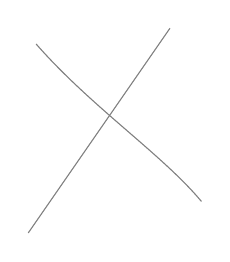
\begin{tikzpicture}\draw[gray] (0,0)--(1.8,2.6);\draw[gray] (0.1,2.4) .. controls (0.8,1.6) and (1.7,1) .. (2.2,0.4);\end{tikzpicture}}
% position: middle quotient
\[E\simeq(E_1\otimes E_2)\oplus(L_1\otimes L_2)/(E_1\otimes L_2)+_{L_1\otimes L_2}(\unsure{E_1|L_1}\otimes E_2)\]
\diagram{\begin{tikzcd}A\times E\arrow[r]&\uline{\unsure{O|0}}\end{tikzcd}}
\unsure{accouplement},
% position: two sequences
\diagram{\begin{tikzcd}
0\arrow[r]&k\arrow[r,dash]&A\arrow[r]&L_1^\vee\otimes L_2^\vee\arrow[r]&0\\
0\arrow[r]&L_1\otimes L_2\arrow[r,dash]&E\arrow[r]&\unsure{k|O}\arrow[r]&0
\end{tikzcd}}
% position: pairing with overwritten arguments
\[
\left\langle
\underset{\substack{\rotatebox{90}{$\in$}\\A_1\otimes A_2}}{\unsure{f_1|x_1}\otimes f_2},
\underset{\substack{\rotatebox{90}{$\in$}\\L_1\otimes L_2}}{\unsure{\deleted{u_1\otimes u_2}\inserted{u}}}
\right\rangle=
\deleted{\unsure{\langle\varphi_1(x_1),u_1\rangle\langle\varphi_2(x_2),u_2}}
\inserted{\underbrace{\varphi_1(f_1)\varphi_2(f_2)}_{\varphi(\unsure{x_1|f_1}\otimes\unsure{x_2|f_2})}\cdot u}
\]
% position: scalar pairings
\[\langle\lambda,x_1\otimes x_2\rangle=\lambda\psi_1(\unsure{x_1})\psi_2(\unsure{x_2})=\lambda\psi(x_1\otimes x_2)\]
\[\langle\lambda,u\rangle=0\]
% position: lower pairing and cancelled fragments
\[\langle f_1\otimes f_2,x_1\otimes x_2\rangle\]
\[\deleted{\unsure{f}}\qquad x\]
\[\deleted{f_1\otimes1}\]
\margin{\deleted{\unsure{expr.} \unsure{bil.} \unsure{en} $\unsure{f_1}\langle f_1,x_1\rangle\langle f_2,x_2\unsure{\rangle}$}
\deleted{\unsure{val} \unsure{sur} $\unsure{A^{\leftrightarrow}|A^{\leftrightarrows}}$, $\unsure{E^{\leftrightarrow}|E^{\leftrightarrows}}$}
$(\deleted{A_1\otimes A_2}\ A_1\unsure{\oplus}A_2,$ \unsure{et} \unsure{sur}}
% position: foot conditions
\unsure{Si} $f\in A_1$ \unsure{ou} $A_2$, \unsure{on} \unsure{veut} \unsure{que} \unsure{ce} \unsure{soit}
\[\unsure{\mathrm{Tr}(f)}\psi(x)\]
\unsure{Si} $x\in E_1\otimes L_2+L_1\otimes E_2$, \unsure{on} \unsure{veut} \unsure{que} \unsure{ce} \unsure{soit}
\[\unsure{\varphi(f)}\cdot\unsure{\pi(x)}\]
\margin{183}

\scanpage{185}
\mspage{496}
% position: top continuation
le déséquilibre marqué par la valorisation exclusive du yang, auquel il m'est
arrivé de faire allusion déjà précédemment (*). La même constatation peut se
faire pour la quasi-totalité des couples yin-yang sur lesquels je suis tombé -
c'est là une chose vraiment très frappante, que je n'avais jamais pris le loisir
précédemment de vérifier de façon aussi circonstanciée.

% position: upper paragraph
Parmi les couples écrits tantôt, le seul qui me semble faire exception
est le couple \mbox{p a s s i o n - s é r é n i t é}, vu que dans l'usage courant\inserted{,}
le mot ``passion'' souvent s'associe à l'image d'un déchaînement, d'une violence,
ou sinon d'un \mbox{l a i s s e r - a l l e r}, avoisinant fâcheusement le nuage
d'associations entourant un mot comme ``\mbox{t u r p i t u d e}''. Comme par hasard,
laisser-aller et turpitude désignent des états de déséquilibre psychique carac-
térisés par une excessive prépondérance \mbox{y i n}, féminine! Et symétriquement,
suivant les mêmes mécanismes pousse-bouton (qui révèlent nos conditionnements
courants, et nullement la nature d'une chose comme la ``sérénité''), le mot ``sé-
rénité'' s'associe (par opposition à ``passion'') à l'image d'un \mbox{c o n t r ô l e}
\mbox{d e\quad s o i} - d'une qualité donc qui, comme de juste, est d'essence \mbox{m a s c u-}
\mbox{l i n e}. (En fait, le pendant yin du ``contrôle'' n'est nullement la ``passion'',
mais ``l'abandon''.)

% position: middle paragraph and displayed pair
Ce qui se passe donc ici, c'est que par suite d'une confusion générale
dans les esprits sur la nature de certaines choses, s'exprimant par une égale
confusion dans l'usage de certains mots, censés les désigner, il y a une con-
fusion du couple yang-yin ``passion-sérénité'' avec l'ensemble des deux notions
\begin{center}relâchement - contrôle,\end{center}
dont les termes sont yin-yang (sans pour autant constituer un ``couple'', les
deux termes en présence n'ayant aucune envie de s'épouser!). Il me semble donc
que la soi-disante ``exception'' à la règle (de la valorisation systématique du
yang) en est au contraire une confirmation particulièrement intéressante! Et
je ne serais pas étonné qu'il en soit de même avec les autres quelques exemples
que j'ai relevés, où dans un couple yang-yin, c'est le terme yin qui semblerait
valorisé.

% position: lower paragraph
Je ne suis d'ailleurs nullement sûr que cette distorsion dans la vision
du monde que je constate dans la civilisation dite ``occidentale'', provenant de ce
parti-pris systématique en faveur du masculin, opposé au féminin - que cette
distorsion, ce déséquilibre soient tellement moindres dans la tradition chinoise,
% position: footnote
\par\noindent\rule{0.24\linewidth}{0.3pt}\par
(*) Voir la note ``Yang enterre yin (1) - ou le muscle et la tripe'', n° 106.
\margin{184}

\scanpage{186}
% position: top four images and involutions
\diagram{\begin{tikzcd}[column sep=small]
1,\arrow[d]&\unsure{u_1},\arrow[d,mapsto]&\unsure{u_2|u_1},\arrow[d,mapsto]&u_{\unsure{2|1}}u_2\arrow[d]\\
2&\unsure{\deleted{2u_1}\inserted{0}},&\unsure{\deleted{2u_2}\inserted{0}}&2u_{\unsure{1|2}}u_{\unsure{2|3}}=v
\end{tikzcd}}
\margin{$\sigma_1\sigma_2$}
\[v\longmapsto2u_{\unsure{2|1}}u_{\unsure{3|2}}\]
\[1\qquad-u_1^2=c_1 1,\quad-u_2^{\unsure{2}}=c_2\cdot1,\quad u_{\unsure{2|1}}^2u_2^2=c_1c_2\]
% position: central diagram
\diagram{\begin{tikzcd}[column sep=large,row sep=large]
 &E_1\otimes E_2\arrow[r]\arrow[rrr,bend left=20,"x_1\otimes x_2\mapsto x_1\otimes x_2+\bar x_1\otimes\bar x_2"]&E_1\wedge E_2\arrow[rr,"?",very thick]&&E_1\otimes E_2\arrow[dd,leftrightarrow,"\unsure{\text{can}}"]\\
 & & & &\\
E_1\otimes_0 E_2\arrow[uur,"\unsure{\text{inc.}}"]\arrow[r,"\pi"']&L_1\otimes L_2\arrow[uur]\arrow[uurrr,bend right=12,"{\substack{u_1\otimes u_2\mapsto u_1\otimes u_2\\\unsure{\text{inc. can.}}}}"']\arrow[rrr,"\mathrm{id}"']&&&L_1\otimes L_2
\end{tikzcd}}
% position: middle left condition
\margin{$\deleted{\unsure{x_1}}$}
\[\underset{\substack{\unsure{\rotatebox{-90}{$\in$}}\\x_1\otimes u_2}}{E_1\otimes L_2}\]
% position: middle computation with insertion
\[\pi_1(x_1)\otimes u_2=(2x_1-T_1\inserted{\psi_1(x_1)})\otimes u_2\]
\[x_1\otimes u_2+(\psi_1(x_1)T_1-x_1)\otimes(-u_2)\]
\[=2x_1\otimes u_2-\psi_1(x_1)T_1\otimes u_2\]
\margin{O K}
% position: lower expansion
\[(x_1+u_1)\unsure{*|\circ}(x_2+u_2)=(\sigma+\bar\sigma)[(x_1+u_1)\otimes\unsure{(x_2|x_2}+u_2)]\]
\[=x_1*x_2+\pi_1(x_1)\otimes u_2+\unsure{u_1}\otimes\pi_2(x_2)+\underbrace{u_1*u_2}_{\substack{\parallel\\2u_1\otimes u_2}}\]
\[b_1\otimes u_2+u_2\otimes b_{\unsure{1|2}}+2u_1\otimes u_2\]
\[\deleted{b_1u_2+b_2u_1+u_1}\]
% position: bottom formula and its images
\diagram{\begin{tikzcd}[column sep=small,row sep=small]
(x_1+u_1)\unsure{\circ|*}(x_2+u_2)\unsure{:|=}&x_1*x_2\arrow[d,mapsto]&+(b_1\underbrace{u_2+b_2u_1+2u_1u_2})&\in E_1\wedge E_2\arrow[d,dash]\\
&x_1*x_2\arrow[d,equal]&&E_1\otimes E_2\\
&\mathrm{Tr}_{E_1\otimes E_2/E_1\wedge E_2}(x_1\otimes x_2)&&
\end{tikzcd}}
\margin{185}

\scanpage{187}
\mspage{500}
% position: top continuation
tant bien que mal. Cette réalité ``sociale'' est le produit d'un conditionnement
immémorial, lequel très tôt prend racine dans le ``moi'' en formation et le struc-
ture. Pourtant, au delà de cette réalité-là, il est une réalité plus profonde,
venant de beaucoup plus loin encore, laquelle est déterminante dans la pulsion
amoureuse elle-même. C'est la réalité d'une \mbox{c o m p l é m e n t a r i t é}
profonde, essentielle des sexes, où il n'y a nulle place pour un quelconque
``antagonisme''. C'est la réalité aussi qui se manifeste clairement dans toutes les
espèces vivantes, à la seule exception de la nôtre, où elle se trouve occultée
dans une large mesure par l'antagonisme culturel, donc par un état de \mbox{d i v i-}
\mbox{s i o n} propre à l'homme et à la société humaine.

% position: long middle paragraph
Les clichés courants romantiques, style ``Nous Deux'', qui dominent une
grande partie de la littérature et des médias, montent d'ailleurs en épingle
une ``complémentarité'' de pacotille, tout en jetant un voile pudique sur le trou-
blant aspect antagoniste homme-femme, ou (au mieux) en le traitant comme une
sorte d'accident un peu piquant, bienvenu pour mettre quelque piment dans un
repas un peu trop fadasse ou sirupeux sinon. Dès qu'on dépasse ce gen\inserted{re de}
clichés rassurants, on se voit aussitôt confronté à la réalité de cet antagonis-
me homme-femme - réalité apparemment universelle, et au surplus d'une tenacité à
toute épreuve, une tenacité de chiendent! Mais \quad partir de cette réalité omni-
présente et irrécusable, pour instituer une sorte d'antagonisme cosmique du
yin et du yang, du ``féminin'' et du ``masculin'', c'est projeter sur l'Univers
entier l'état de déchirement, de division profonde de la société humaine et de
la personne, une maladie donc propre à notre espèce. C'est aussi perpétuer sa
propre ignorance d'une \mbox{a u t r e} réalité en soi-même (rejoignant cette
réalité cosmique de l'harmonie des complémentaires), d'une réalité toute aussi
tenace (ou, pour mieux dire, indestructible), mais plus cachée. Cette réalité
va à l'encontre des conditionnements instituant tacitement un antagonisme de
fait aussi bien entre la femme et l'homme, l'épouse et l'époux, qu'entre cela
en nous-même qui est ``femme'' et ce qui est ``homme''.

% position: lower paragraph
A vrai dire, cette vision \mbox{d u a l i s t e} ou \mbox{g u e r r i è r e} de
l'Univers, où un aspect des choses se trouverait en guerre constante avec un
aspect ``symétrique'' tout aussi essentiel - cette vision n'est nullement le
fruit d'une \mbox{r é f l e x i o n}, qui ``partirait'' (comme j'écrivais à l'instant)
de la réalité du conflit dans le couple humain et dans la société humaine, pour
la ``déduire'' ensuite (ou ``l'instituer'', comme j'écrivais plus justement) dans
le Cosmos tout entier. Elle n'est ni plus, ni moins que l'expression fidèle,
automatique autant dire, du conditionnement culturel, et va dans le sens d'une
\margin{-}
\margin{186}

\scanpage{188}
% position: heading and unfinished pairing
\unsure{Considérons}
\[\langle u_1*u_2,x_1*x_2\rangle=\]
\margin{$\deleted{x_1*x_2}$}
% position: upper branching diagram
\diagram{\begin{tikzcd}[row sep=small]
 &A_1\otimes A_2\unsure{\cdot}\oplus(A_1\oplus_{\unsure{0|O}}A_2)\arrow[d]\\
A_1\otimes A_2\arrow[ur]&A
\end{tikzcd}}
% position: upper middle sequence and cancelled lower object
\diagram{\begin{tikzcd}
A_1\otimes A_2\arrow[r,"\unsure{\text{inj}}"]&(A_1\otimes A_2)\oplus(A_1\oplus_{\uline{\unsure{O|0}}}A_2)\arrow[r,"\unsure{\text{surj}}"]&A\\
&\deleted{E_1\otimes E_2}\arrow[r,dash]&E
\end{tikzcd}}
% position: middle cancellations
\[\deleted{A\simeq A_1\otimes A_2\times\uline{\unsure{O|k}}\oplus\unsure{A_1\oplus A_2}}/\mathrm{Im}(A_1\oplus_k A_2)\]
\deleted{$\unsure{E^\vee|A^\vee}\simeq$ \unsure{Formes} \unsure{bilin} \unsure{sur} $\unsure{E_1|A_1}\times\unsure{A_2|E_2}$ \unsure{telles} \unsure{que}}
% position: middle dual and brace
\[A^\vee\simeq(f,\deleted{\unsure{g_1,g_2}}\inserted{\lambda})\]
\unsure{avec}
\diagram{$\left\{\begin{array}{l}
f\ \unsure{\text{forme}}\ \text{bil.}\ \unsure{\text{sur}}\ A_1\times A_2\longrightarrow k\\
\deleted{\unsure{g_1:\varphi A_1\mathrel{-} k}}\\
\deleted{g_2:A_2\longrightarrow k}
\end{array}\right.\qquad\lambda\in k$}
% position: lower left condition words
\unsure{satisfaisant}
\deleted{\unsure{les} \unsure{équations}}
% position: cancelled condition a and its continuation
\deleted{a) $g_1(1)=g_2(1)$ \unsure{i.e.} $g$ \unsure{provient} \unsure{d'une}}
\unsure{forme} \unsure{sur}
\diagram{\begin{tikzcd}[row sep=small]
A_1+A_2\arrow[dr,bend right=10]&\subset A_1\otimes A_2\\
&k
\end{tikzcd}}
% position: cancelled condition b
\deleted{b) $f|(A_1+A_2)=\uuline{2}g$ \unsure{i.e.}}
\[\deleted{f(x_1,1)=2g_1}\]
\[\deleted{f(\unsure{1},x_2)=2g_2}\]
\[\unsure{u_1|x_1}\in A_1\qquad\unsure{u_2|x_2}\in A_2\]
% position: lower left trace conditions
\[f(\unsure{x_1})=\lambda\mathrm{Tr}_1(x_1)\]
\[f(x_2)=\lambda\mathrm{Tr}_2(x_2)\]
% position: foot sequence
\diagram{\begin{tikzcd}[row sep=small]
\unsure{0|\cdot}\arrow[r,dash]&L_1\otimes L_2\arrow[r,dash]&E\arrow[r,"\psi"]&\unsure{O|0}\arrow[r]&0\\
&&\rotatebox{-90}{$\in$}&&\\
&&x&&
\end{tikzcd}}
\diagram{\begin{tikzcd}\deleted{E}\arrow[r]&\deleted{A^\vee\unsure{?}}\end{tikzcd}}
\[\deleted{\lambda=\unsure{\psi(x)}}\qquad E\]
\margin{187}

\scanpage{189}
\mspage{497}
% position: top continuation
\texttt{ou même dans le monde chinois (ou plus généralement le monde ``oriental'') d'au-
jourd'hui. Aucun signe, au niveau de la vie de tous les jours, ne pourrait me le}
faire supposer, ni à travers mes amis et amies orientaux, ni à travers les échos
qui ont pu me parvenir de la tradition et de la vie d' aujourd'hui dans la
Chine ou d'autres pays d'extrême-Orient - bien au contraire. Il me semble plutôt
qu'une fine perception du dynamisme yin-yang s'est cantonnée à peu près exclu-
sivement dans la \mbox{p r a t i q u e} de \mbox{c e r t a i n s\quad a r t s} - comme
la calligraphie, la poésie, l'art culinaire et, bien entendu, l'art médical (*).

% position: middle paragraph
C'est le dernier surtout, sous le nom de ``médecine chinoise'' et par le
biais de certains succés spectaculaires de l'acupuncture, qui a fini au cours \unsure{des}
vingt ans passés, par acquérir droit de cité chez nous, et à être investi de
prestige. Nombreux pourtant sont encore ceux qui ignorent qu'en médecine chi-
noise, l'alpha et l'oméga de l'appréhension du corps, de la circulation d'éner-
gie dans le corps et des perturbations de celle-ci (qui constituent les états
morbides que nous appelons ``maladies''), se trouve justement dans une dialecti-
que très fine du yin et du yang. Le fait que cette dialectique ``marche'', puis-
que la ``médecine chinoise'' basée sur elle est efficace (y compris dans de nom-
breux cas qui échappent aux moyens de la panoplie occidentale), peut être con-
sidéré comme une sorte de ``preuve'' de la réalité des ``principes'' ou ``aspects''
ou ``modes'' (d'appréhension, ou d'existence) yin et yang - que ce ne sont pas
de pures spéculations sorties des chapeaux de certains philosophes et autres
poètes (pour ne pas dire fumistes).

% position: lower paragraph
On peut se demander, il est vrai, quel est le sens de telles preuves, et
même de toute ``preuve'' quelle qu'elle soit de la validité de telle ou telle
vision du monde. A supposer même que la preuve ait convaincu (c'est-à-dire,
que l'intéressé ait bien voulu se laisser convaincre), et même et par dessus
le marché\unsure{\inserted{,}} que la vision en question soit profonde et par là\unsure{\inserted{,}} bienfaisante -
la meilleure preuve du monde est impuissante pourtant à \mbox{c o m m u n i q u e r}
% position: footnote
\par\noindent\rule{0.24\linewidth}{0.3pt}\par
(*) (21 octobre) J'ai oublié dans le nombre l'\mbox{a r t\quad d i v i n a t o i r e},
dans le \mbox{Y i\quad K i n g} ou ``livre des changes'', qui jouit aujourd'hui d'une\unsure{.} grande
popularité dans certains milieux tant en Europe qu'en Amérique. Les \unsure{$\cdot$}64 ``hexagram\unsure{-}
mes'' qui constituent les ``mots'' de base du langage divinatoire du Yi King, ne \unsure{son|sont}
autres que les $2^{\inserted{6}}$ combinaisons possibles de suites de six ``signes'' yin et yang,
depuis le yin pur (six répétitions du yin ) au yang pur (six répétitions du \unsure{yang|yang)}
Il semble y avoir là une sorte d'alchimie d'une grande finesse des combinaisons
du yin et du yang, qui \inserted{(}paraît-il\inserted{)} avait fasciné Jung. L'intérêt de cette alchimie
\inserted{(}en tant que ``collection d'archétypes'' notamment) me paraît a priori indépendant
de son usage en art divinatoire, et du crédit qu'on est disposé à accorder à
un tel usage.
\margin{188}

\scanpage{190}
% position: heading and crossed opening
\deleted{\unsure{E}}
$u$ \unsure{décrit|déduit} en termes de $u_1,u_2$ ?

\deleted{$\unsure{u\simeq u_1}$ \unsure{Comment}}
\unsure{Comment} \deleted{\unsure{calculer}}
On doit avoir
% position: upper product trace and norm
\[u_1\overset{\unsure{\leftrightarrow|\leftrightarrows}}{*}u_2=\uline{\lambda}u+\uline{\mu}\qquad\text{avec }\lambda,\mu\]
\[\unsure{\mathrm{Tr}e|\mathrm{Tr}}_{A/k}(u_1*u_2)=-\deleted{\unsure{u}}\lambda\beta+2\mu\]
\[\mathrm{N}_{A/k}(u_1*u_2)=\uline{\lambda^2}c+\uline{\mu^2}\unsure{-|+}\uline{\lambda\mu}\beta\]
% position: middle left cancellation
\[\deleted{\unsure{\mathrm{Tr}|\Pi}_{A_1\otimes A_2}}\]
% position: middle bases and pairings
base de $A$\qquad $1,u$

base \inserted{duale} de $E$\qquad
$\deleted{\unsure{E}e_1\otimes e_2,\;x=x_1*x_2}$
\[x=x_1*x_2,\quad e=e_1\otimes e_2\]
\diagram{$\begin{array}{ll}
\langle1,x\rangle=1&\langle1,\unsure{u|e}\rangle=0\\
\langle\unsure{u},e\rangle=1&\langle u,x\rangle=0
\end{array}$}
% position: lower left coefficient pairings
\[\lambda=\deleted{\langle u,e\rangle}\langle u_1*u_2,\overbrace{e_1\otimes e_2}^{e}\rangle\]
\[\mu=\langle u_1*u_2,\underbrace{x_1\unsure{*|\otimes}x_2}_{x}\rangle\]
\[u_1*u_2\]
% position: lower right small field line
\diagram{\begin{tikzcd}\unsure{\mathbb F_2}\arrow[r,dash]&\unsure{\mathbb F_2}\times\unsure{\mathbb F_2}\end{tikzcd}}
% position: lower right paired diagrams with circled arrows
\diagram{\begin{tikzcd}[column sep=large,row sep=large,execute at end picture={
\draw ($ (\tikzcdmatrixname-1-2.east)!0.5!(\tikzcdmatrixname-1-3.west)+(0,0.05) $) ellipse[x radius=0.86cm,y radius=0.30cm];
}]
A_1\otimes A_2\arrow[r,"*"]\arrow[rr,bend left=30,"\deleted{x_1\otimes x_2}"]&A\arrow[r,"\overset{(\unsure{I|II})}{\unsure{\leftrightarrow|\leftrightarrows}}"]&A_1\otimes A_2\\
\overset{\times}{E_1\otimes E_2}\arrow[d]&\overset{\times}{E}\arrow[l,"\unsure{\leftrightarrow|\leftrightarrows}"]\arrow[d]&\unsure{\deleted{A_1}\inserted{E_1}}\otimes E_2\arrow[l,"{\text{\textcircled{$*$}}}"]\arrow[d]\\
\uline{\unsure{O|0}}&\unsure{O|0}&\uline{\unsure{O|0}}
\end{tikzcd}}
% position: low crossed map and transpose identity
\[\deleted{\unsure{(x,y)\longmapsto x\otimes y,\;x*}}\]
\[{}^t(\mathrm{id}+\unsure{\sigma_1}\otimes\sigma_2)=\mathrm{id}+\underset{\substack{\parallel\\\sigma_1}}{({}^t\sigma_1)}\otimes\underset{\substack{\parallel\\\sigma_2}}{{}^t\sigma_2)}\]
% position: foot definition and cancellations
\deleted{$\unsure{u}$}\qquad\deleted{$u_1\otimes u_2$}

$u\in A$ \unsure{défini} \unsure{par}
\diagram{$\left\{\begin{array}{l}
\langle u,e_1\otimes e_{\unsure{1|2}}\rangle=1\\
\langle u,x_1*x_2\rangle=0
\end{array}\right.$}
\margin{189}

\scanpage{191}
\mspage{498}
% position: upper continuation
\mbox{u n e}\quad\mbox{v i s i o n}, et encore moins une vision du monde. Cela vous fait une
belle jambe d'être ``convaincu'' mordicus d'une vision qui reste étrangère, incom-
prise. Pour tout dire, cela n'a pas même de sens - ou plus exactement, le vrai
sens de sa ``conviction'' n'est pas plus compris par l'intéressé, que cette vision
qu'il fait mine d'incorporer à son lourd bagage culturel.

% position: upper middle paragraph
Quand la vision est comprise et assimilée, la question même d'une ``preuve''
apparaît étrangement saugrenue - un peu comme de prouver que le ciel est bleu
quand on voit bien qu'il est bleu, ou que le parfum d'une fleur qu'on aime est
bon...
\margin{\figure{\begin{tikzpicture}\draw[gray] (0,0) .. controls (-0.5,-0.4) and (-0.8,-1.1) .. (-0.8,-1.7);\end{tikzpicture}}}
% position: lower main paragraph
($^{112}$) (17 octobre) Mes premières réflexions sur le double aspect ``féminin'' et
``masculin'' sont issues d'une réflexion sur moi-même. C'était vers les débuts
1979, à un moment où j'ignorais encore les mots chinois ``yin'' et ``yang'', et
l'existence d'une sorte de ``philosophie'' subtile du jeu incessant du yin et
du yang, dans la tradition culturelle chinoise. J'ai appris la chose vers la
fin de la même année je crois, par ma fille et surtout par mon gendre Ahmed, qui
commençait alors à s'intéresser à la médecine chinoise, sur laquelle il a accro-
ché fortement dans les années suivantes. La plupart de ce qu'il me disait re-
coupait et confirmait la vision à laquelle j'étais parvenu, chose qui n'avait
rien pour me surprendre. Si surprise il y avait, c'était plutôt dans les quel-
ques cas de ``couples'' où le rôle yin-yang ``naturel'' me semblait renversé, dans
la tradition chinoise. Mon réflexe (fortement ``yang'' en l'occurence!) avait été
une conviction à fleur de peau que ce ``renversement'' devait être dû à une dé-
formation culturelle, sans d'ailleurs aller y regarder de trop près (*) - \unsure{c'étai|c'était}
à un moment où mes gammes passées sur le féminin-masculin me paraissaient bien
lointaines, alors que j'étais engagé dans une méditation autrement plus \unsure{personel|personelle}
% position: footnote rule and footnote
\par\noindent\rule{0.24\linewidth}{0.4pt}\par
(*) Cette réaction d'assurance péremptoire, vis-à-vis d'une tradition millénai-
re qui aurait pu m'inciter à plus de prudence, est celle-là même qui, enfant,
m'a fait récuser la formule (bien compliquée ma foi!) $\inserted{\pi}=3,14\ldots$ enseignée par
les livres, en faveur de $\inserted{\pi}=3$ dont je m'étais convaincu par mes propres moyens.
(Voir la note ``La quadrature du cercle'', n° 69.) Il est vrai que pour cette his-
toire du yin et du yang, j'avais eu ample occasion de me rendre compte à quel
point l'appréhension de la nature du ``féminin'' et du ``masculin'', et de leurs
interrelations, est faussée par des distortions culturelles invétérées, d'une
force considérable. Je ne me rendais pas compte encore, par contre, à quel point
aussi une appréhension précise et délicate de ces relations était chose \unsure{essentie|essentiel}le
dans la pratique de certains arts traditionnels chinois, et poussé à un degré
de grande finesse.
% position: lower left strokes and number
\margin{$-$}
\figure{\begin{tikzpicture}\draw[gray!50] (0,0)--(1.8,0.5);\end{tikzpicture}}
\margin{190}

\scanpage{192}
% position: upper left defining quadratics
\diagram{$\begin{array}{ll}
u_1&u_1^2+b_1u_1+c_1=0\\
u_2&u_2^2\unsure{+}b_2u_2\unsure{+}c_2=0
\end{array}$}
% position: upper product expansion
\[u_1*u_2=u_1\otimes u_2+(u_1+b_1)\otimes(u_2+b_2)=2u_1u_2+b_2u_1+b_1u_2+\uuline{b_1b_2}\]
% position: upper prose and overwritten line
\unsure{ne|en} \unsure{forme} \unsure{ainsi} une \unsure{base} de
\deleted{\unsure{A'} \unsure{par} \unsure{déf.} \unsure{ici}}
$A$: avec $1$ \unsure{ça} \unsure{croule} si $2=0,\ b_1=b_2=0$
% position: middle direct sums
\[A_1\simeq\uline{\unsure{O|0}}\oplus\uline{L}_1^\vee\qquad A_2=\uline{\unsure{O|0}}\oplus L_2^\vee\]
\[E_1\unsure{\simeq|\in}\unsure{O|0}\unsure{+|\oplus}L_1,\quad E_2\simeq\uline{\unsure{O|0}}+L_2\]
% position: middle right sequence and elements
\diagram{\begin{tikzcd}[column sep=small,row sep=small]
E_1\otimes E_2\arrow[r,dash]&E_1\wedge E_2\arrow[r,dash]&E_1\otimes E_2\\
x_1\otimes x_2&x_1\unsure{\deleted{\otimes}\inserted{*}}x_2&\mathrm{Tr}_{\unsure{1}}(x_1\otimes x_2)
\end{tikzcd}}
% position: middle left cancelled and rewritten algebra
\[\deleted{A\simeq\unsure{L_1^\vee}\otimes L_2^\vee\unsure{+}}\]
\[A\simeq\uline{\unsure{O|0}}\unsure{\oplus|\otimes}L_1^\vee\otimes L_2^\vee\]
\diagram{$\begin{array}{ll}
e_1\in L_1&e_2\in L_2\\
\unsure{\text{base}}\ \text{de }L_1&\unsure{\text{base}}\ \text{de }\unsure{L_2|e_2}
\end{array}$}
% position: middle isolated mark and coefficients
\[\unsure{x}\]
\diagram{$\begin{array}{ll}
b_1=\beta_1e_1&c_1=\gamma_1e_1^{\unsure{\otimes2|2}}\\
b_2=\beta_2e_2&c_2=\gamma_2e_2^{\unsure{\otimes2|2}}
\end{array}$}
% position: lower left basis and dual basis
\[A\simeq\uline{\unsure{O|0}}+\underset{\deleted{\unsure{x}}}{\unsure{\uline{O}}e_1^*}\]
\[u_1=e_1^*\qquad u_2=e_2^{\unsure{*|'}}\]
% position: lower cancelled quadratics
\[\deleted{u_1^2+\beta_1u_1\unsure{=|-}e_1^*}\]
\[\deleted{\unsure{u_1^2+(\beta_1e_1)u_1}}\]
% position: lower live quadratics and unfinished expression
\[u_1^2+\beta_1u_1+\gamma_1=0\]
\[u_2^2\unsure{+|=}\beta_{\unsure{1|2}}u_2+\gamma_2=0\]
\[u=\unsure{2}uu'+\]
% position: lower first correspondence and defining brace
\diagram{\begin{tikzcd}
x_1,e_1\arrow[r,leftrightarrow]&u_1\in A_1\qquad u_1^2+\beta_1u_1+\gamma_1=0
\end{tikzcd}}
\unsure{\deleted{Alors}}
\diagram{$\left\{\begin{array}{l}
e_1=\varphi(u_1)\\
\langle\unsure{u_1},\unsure{\deleted{=}}x_1\rangle=0\\
\psi(x_1)=1
\end{array}\right.$}
% position: foot second correspondence
\diagram{\begin{tikzcd}
(x_2,e_2)&u_2\in A_2\ \Big|\ u_2^2+\beta_2u_2+\gamma_{\unsure{2|1}}=0\arrow[l]
\end{tikzcd}}
% position: foot product correspondence and final quadratic
\diagram{\begin{tikzcd}
(x_1*x_2,e_1\otimes e_2)\arrow[r,leftrightarrow]&u\in A.
\end{tikzcd}}
\[u^2+\beta u+\gamma=0\]
\margin{191}

\scanpage{193}
\mspage{499}
% position: upper continuation
le sur la vie de mes parents et sur mon enfance. C'est des mois ou des années \unsure{plu|plus}
tard seulement, je crois, que par un certain nombre de recoupements, je me suis
rendu compte que dans certains cas mon appréhension des rôles yin et yang dans
tels ou tels ``couples'' était resté un tantinet superficielle; que j'avais mis \unsure{da|dans}
le même sac, un peu hâtivement, des situations de nature différente que la \unsure{dialec|dialec-}
tique yin-yang chinoise prenait bien soin de distinguer ($112^{\unsure{\inserted{\prime}|\inserted{1}}}$). Maintenant, je \unsure{me}
rends compte que l'appréhension du yin et du yang reste encore relativement gros-
sière et statique chez moi, surtout si on la compare à la finesse requise pour
l'exercice de certains arts traditionnels chinois comme la médecine (intimement
liée aussi à la diététique et à l'art culinaire), où cette appréhension finit \unsure{par}
devenir comme une seconde nature.

% position: middle paragraph
J'ai eu l'impression plus d'une fois que chez les pratiquants et praticiens
de ces arts, qu'ils soient orientaux ou européens, cette finesse d'appréhension
reste fragmentaire, en ce sens qu'elle reste, dans une très large mesure, soi-
gneusement cantonnée dans l'exercice de cet art. Dans la vie de tous les jours,
elle agirait plutôt comme un ``savoir'' ordinaire, se superposant purement et sim-
plement au ``savoir'' du conditionnement culturel (et autre), et restant plus ou
moins lettre morte vis-à-vis de celui-ci. Pour le dire autrement, j'ai eu l'im-
pression que la vision du monde et de soi, et les mécanismes de répression dans
la perception de la réalité, ne sont en rien différents chez ces personnes tout
ce qu'il y a d'``averties'', que chez le commun des mortels.

% position: lower middle paragraph
Cette impression se recoupe avec une autre, que j'ai eue en parcourant deux
ou trois textes, écrits par des européens censés être ``dans le coup'', qui se
proposent de donner un aperçu de la philosophie traditionelle chinoise du yin
et du yang. (L'un des auteurs est un orientaliste français bien connu, dont
le nom m'échappe à présent.) La chose qui m'a frappée, c'est que dans ces textes,
le yin et le yang sont présentés comme des principes ``\mbox{o p p o s é s}'' (ou
``\mbox{c o n t r a i r e s}'' ) voire \mbox{a n t a g o n i s t e s} (ce dernier terme
revient à plusieurs reprises dans un de ces textes), plutôt que \mbox{c o m p l é -}
\mbox{m e n t a i r e s}. Cette ``opposition'' ou ``antagonime'' aurait son expression
typique dans celui qui aurait lieu entre la femme et l'homme à l'intérieur de
la société humaine, et à l'intérieur du couple institué par la société.

% position: bottom paragraph
L'antagonisme dans le couple époux-épouse est bel et bien une réalité,
aussi bien à l'Est qu'à l'Ouest. Elle est profondément enracinée dans la cul-
ture, à tel point qu'il peut paraître parfois comme un des aspects (parfois
déroutant!) de la condition humaine, voire même comme la racine du conflit en
l'homme ou dans la société humaine. La réalité de cet antagonisme est irrécu-
sable, et elle dépasse certes les clichés courants qui s'efforcent de l'exorciser
\margin{192}
